\chapter{肌肉驱动的步行} \label{chap:chap11}

我们将永不停止探索,而我们所有探索的终点,将是回到我们出发的地方,并第一次了解这个地方。
\begin{flushright}
	——T.S.艾略特
\end{flushright}


\begin{figure}[!htb]
	\centering
	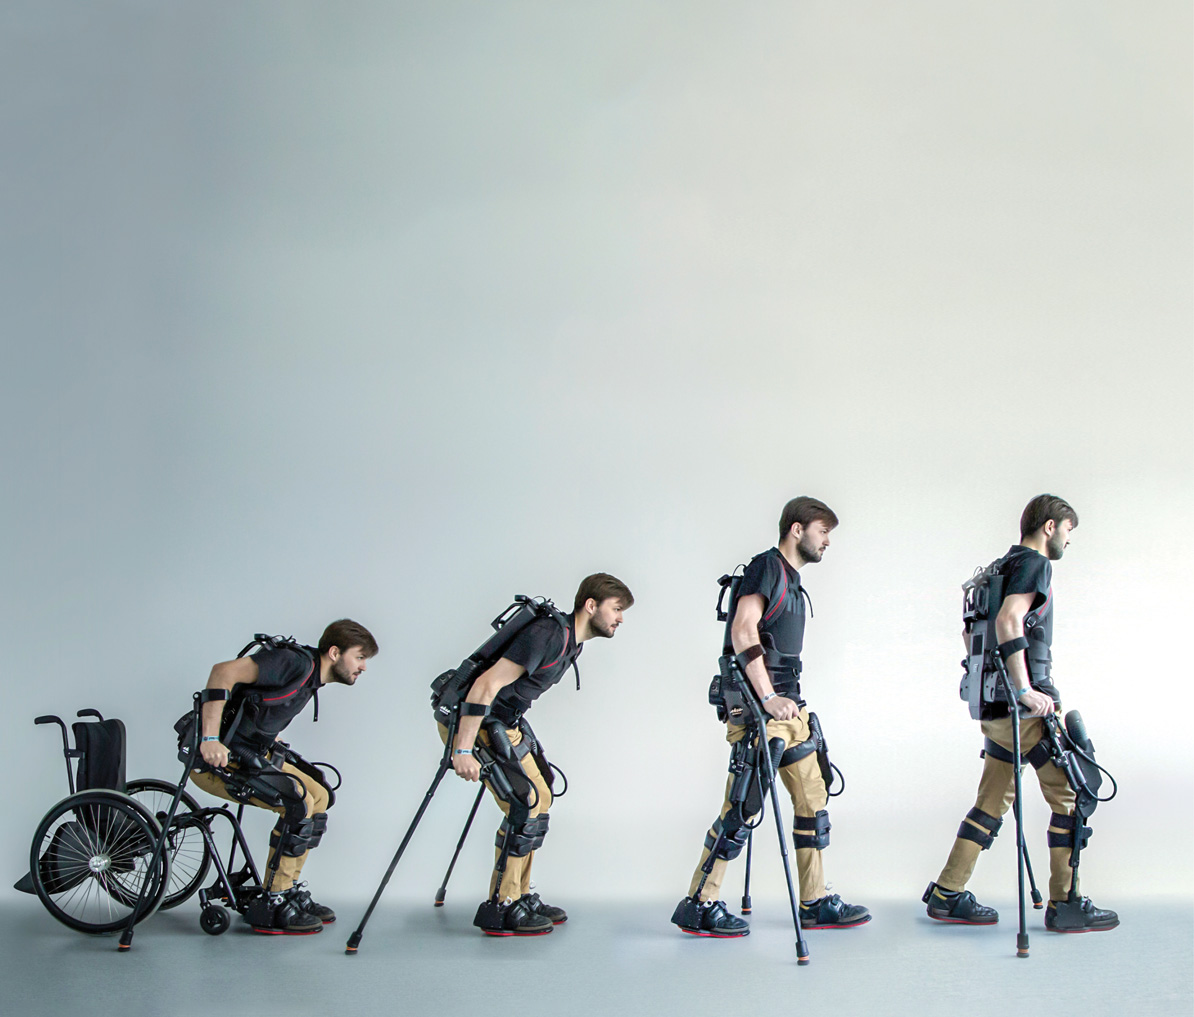
\includegraphics[width=1.0\linewidth]{chap11/11_0}
	% 加星号(*)表示不加编号
	\caption*{ \label{fig:11_0}}
\end{figure}


视频结束,灯光再次闪烁亮起。
没有人知道该怎么办。
视频中,一个13岁的女孩在我们的步态实验室里来回走动。
这个女孩早产六周,被诊断为脑瘫。
她 3 岁开始走路,现在步态是蹲伏的。
由于关节负荷过重,她的膝盖疼痛难忍,而且在平地上行走比其他孩子跑楼梯消耗的能量更多。
由于走路时髋部和膝盖弯曲,她比大多数同龄人矮 20 厘米。
我和同事们正在回顾她的视频,想制定改善她步态的策略,但我们无法就最佳方案达成一致。
除了视频,我们还审阅了步态实验室出具的一份 20 页的报告,报告显示她的关节角度、关节力矩​​和肌电图模式与典型步态不同,但我们仍然不知道是什么导致了她的蹲伏步态。
是腘绳肌紧张吗?
跖屈肌无力?
髋屈肌紧张?
如果我们能找到她蹲伏步态的根本原因,就能建议她进行物理治疗、佩戴腿部支架或进行矫形手术来解决这些问题。


我职业生涯的前 15 年,一直在与其他专家合作,致力于探究脑瘫儿童运动异常的病因。
我们利用所有可用的信息,竭尽全力制定能够改善他们行走能力的治疗方案。
希望依然存在。
大约一半的儿童在手术后病情显著好转。
不幸的是,许多儿童的病情并没有好转,有些甚至恶化了。
开发更佳治疗方法存在一个根本障碍:我们不知道在典型步态中,各个肌肉在产生关节运动方面的作用,也不知道这些作用在脑瘫儿童身上有何不同。
这促使我开发工具,帮助我们更好地理解行走过程中肌肉的活动。


本书到目前为止,我们已经探索了肌肉的形态、功能和模拟。
现在,我们回到最初的起点,怀着理解行走的渴望,并借助新的工具来加深理解。
在第~\ref{chap:chap2}~章中,我们使用仅包含几个代表腿部的机械连杆的模型分析了行走。
虽然这些简单的模型很有价值,但它们并不能帮助我们确定单个肌肉的动作。
腿部肌肉能够产生力量,防止我们摔倒,并在行走时推动我们前进。
肌肉使我们能够背负背包、改变行走速度,以及从步行过渡到跑步。


在本章中,我们将了解肌肉如何协调以产生典型的步行,以及步行的动态如何随速度而变化。
我们还将了解肌肉协调性差为何会导致非典型模式,例如膝关节僵硬步态和蹲伏步态,以及在肌肉协调性受损的情况下如何改善步行动态。


肌肉驱动模拟的一个重要用途是扩展从实验中获得的洞见。
例如,虽然可以测量肌肉活动、地面反作用力和关节运动,但仅靠实验不足以确定每块肌肉如何对地面反作用力和身体运动产生影响。
这就是为什么我们无法确定视频中的女孩为何以蹲伏的步态行走。
我们识别出了异常的肌肉活动和异常运动,但无法确定是哪些肌肉导致了这些异常运动。
肌肉驱动模拟揭示了肌肉引起的运动,并为理解运动过程中的肌肉动作提供了强有力的工具。
在本章中,我们将学习如何构建、测试和分析肌肉驱动的步行模拟。


\section{构建和测试步行模拟}

为了构建行走模拟,我们通常首先记录受试者在测力板上行走时身体各部分的运动和地面反作用力。
我们也可能测量其他量,例如使用肌电图测量肌肉活动,或使用间接量热法测量全身能量消耗。
然后,我们根据测量到的解剖标志位置,定制一个通用的肌肉骨骼模型,使其与受试者的尺寸和形状相匹配。
我们使用逆运动学算法计算行走过程中的关节角度,该算法最小化测量到的标记位置与模型上相应标记在每个时间帧上的位置之间的差异,如第~\ref{chap:chap7}~章所述。
我们模拟跟踪测量运动所需的肌肉激活和力量,如第~\ref{chap:chap10}~章所述,从而生成肌肉驱动的行走模拟(图~\ref{fig:11_1})。
然后,必须评估模拟的准确性,如 Liu 等人(2008 年)和 Hicks 等人(2015 年)的详细描述。
例如,我们可以将模拟肌肉激活与肌电图测量值进行比较,或者将所有模拟肌肉消耗的总代谢能量与全身代谢成本的测量值进行比较。


\begin{figure}[!htb]
	\centering
	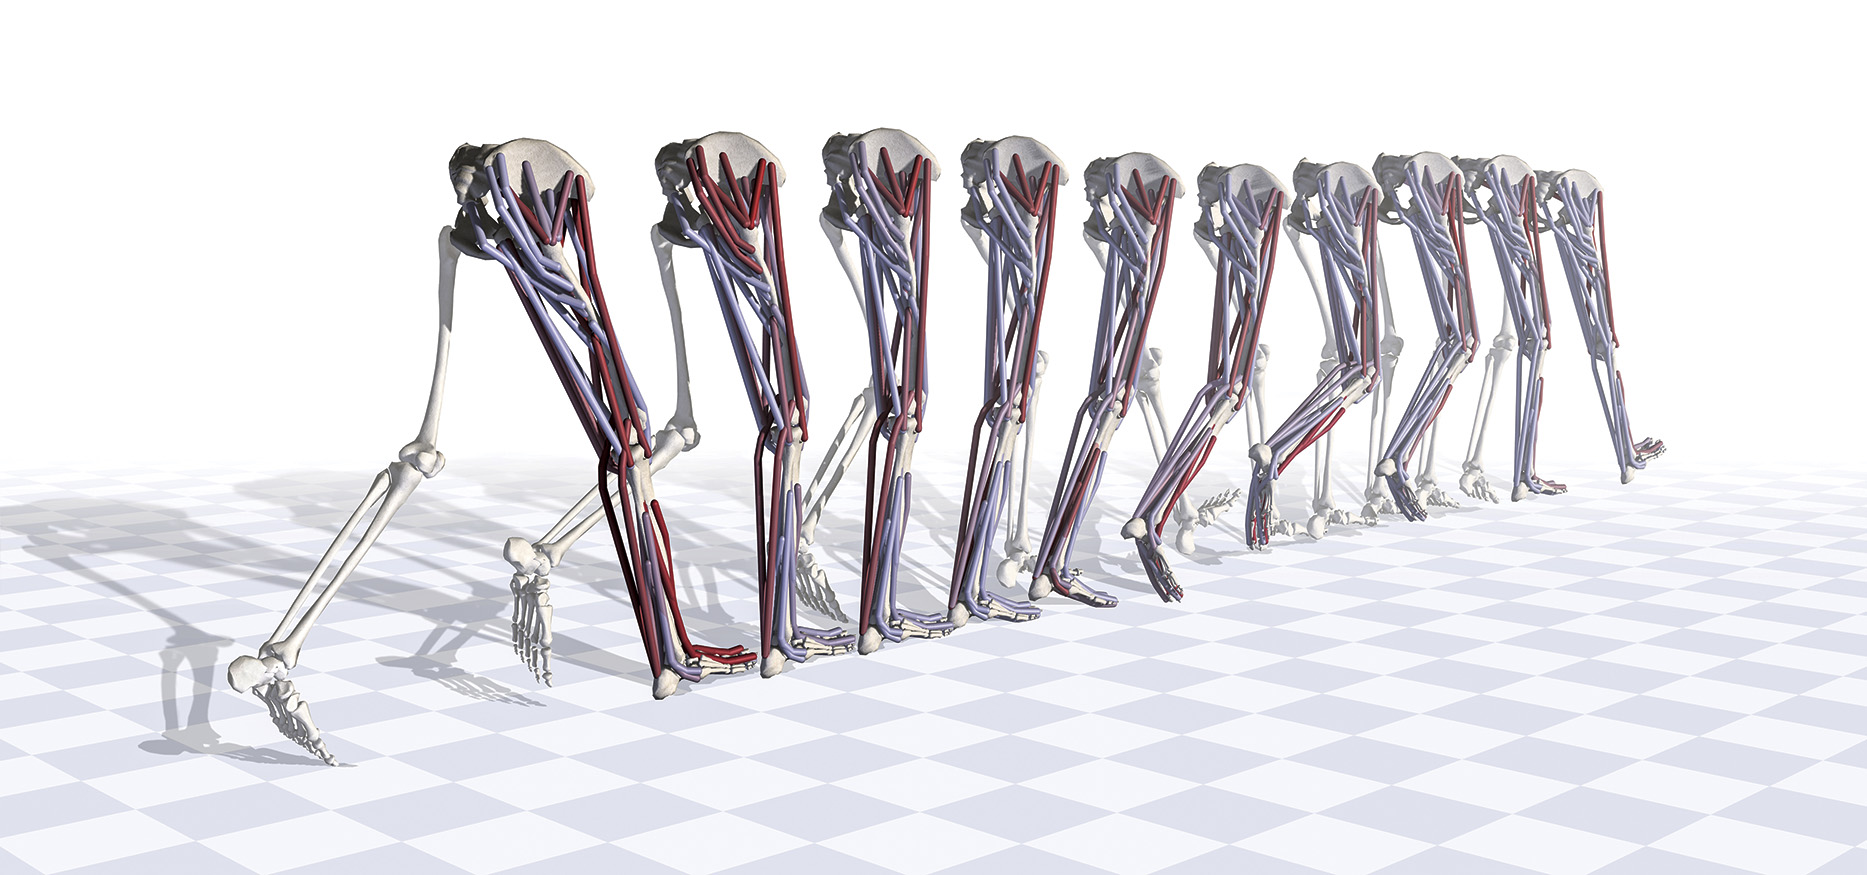
\includegraphics[width=1.0\linewidth]{chap11/11_1}
	\caption{肌肉驱动步行模拟的可视化。
		肌肉的颜色表示其激活程度,范围从非活跃状态(蓝色)到高度活跃状态(红色)。
		数据来自 Dembia 等人(2017)。 \label{fig:11_1}}
\end{figure}


一旦测试了模拟的准确性,我们就可以对其进行分析,以确定肌肉如何影响身体重心的垂直和前后加速度,以及关节和身体各部分的运动。
在过去的 30 年里,我的研究小组使用这种方法分析了数千个由肌肉驱动的人类步态模拟,包括不同速度下的健康和受损步行。
这些分析使我们能够对肌肉如何参与支撑和进展形成一个相当完整的图景。
我总结了我们的主要发现。


\section{肌肉对地面反作用力的贡献}

在站立阶段,肌肉会产生支撑身体重量并调节向前移动的力量。
我们可以通过确定肌肉如何影响重心的垂直加速度来量化肌肉对体重支撑的贡献。
同样,我们可以通过分析肌肉在前后方向产生重心加速度方面的作用来研究肌肉如何促进向前移动。
回想一下,行走过程中身体重心的加速度与地面反作用力除以身体质量有关(公式~\ref{eq:2_2});
因此,分析地面反作用力类似于分析重心加速度。
还要回想一下,地面反作用力是由肌肉“作用”力产生的,并且可以归因于肌肉“作用”力。


在行走时提供体重支撑的肌肉也调节向前移动。
例如,斯坦福大学由 May Liu 领导的研究小组发现,股四头肌和臀大肌在站立初期对支撑做出重要贡献,同时股四头肌也会降低身体的前进速度(图~\ref{fig:11_2})。
臀中肌在站立中期提供支撑,并在站立的后半段有助于向前加速。
比目鱼肌和腓肠肌有助于站立后期的垂直和向前加速。
比目鱼肌和腓肠肌对体重支撑的贡献非常重要,以至于这些肌肉的无力可能会导致蹲伏步态。
正是由于这个原因,在某些情况下,可以通过佩戴可产生跖屈力矩的弹簧式踝关节支架来改善蹲伏步态。


\begin{figure}[!htb]
	\centering
	\includegraphics[width=1.0\linewidth]{chap11/11_2}
	\caption{臀中肌、股四头肌、比目鱼肌、臀大肌和腓肠肌在支撑期的活动。
		股四头肌在支撑初期最为活跃,此时它们加速重心向上和向后移动;
		跖屈肌在支撑后期最为活跃,此时它们加速重心向上和向前移动。
		臀中肌、臀大肌和骨骼排列对体重支撑起着重要作用。
		数据来自刘等人(2008)。 \label{fig:11_2}}
\end{figure}

在站立的短时间内,身体重心会以接近 9.8 米/秒$^2$ 的速度向下加速。
如果没有肌肉力量,身体在这些时间段内几乎处于自由落体状态。
然而,当脚平放在地面上且膝盖接近完全伸展时,由于骨骼对重力提供了被动抵抗(参见图~\ref{fig:11_2}~中的骨骼排列),重心在重力作用下的垂直加速度小于 9.8 米/秒$^2$。
然而,骨骼的被动支撑不足以防止腿部屈曲和塌陷。
在正常行走过程中,肌肉是支撑身体重量的必需品。


将站立肢肌肉对地面反作用力的贡献相加,可以得出类似于我们熟悉的地面反作用力矢量的模式(图~\ref{fig:11_3})。
这表明,在行走过程中,肌肉主要负责产生地面反作用力,从而支撑身体的重量。
总地面反作用力与肌肉产生的地面反作用力之间的差异可以归因于骨骼排列,或者说骨骼对重力引起的向下加速度提供的阻力。
在双支撑过程中,双肢的肌肉都有助于支撑身体的重量;
然而,后肢的肌肉有助于向前移动,而前肢的肌肉则阻碍向前移动(图~\ref{fig:2_5})。


\begin{figure}[!htb]
	\centering
	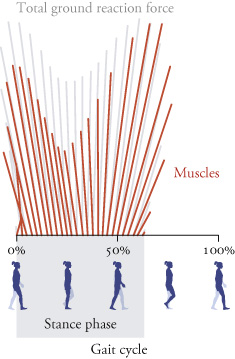
\includegraphics[width=0.4\linewidth]{chap11/11_3}
	\caption{站立肢肌肉(红色)对地面反作用力的贡献与测量到的地面反作用力(灰色)的相对关系。
		两者之差代表骨骼排列的贡献。
		改编自 Liu 等人 (2008)。 \label{fig:11_3}}
\end{figure}


\section{摆动阶段的肌肉动作}

摆动期始于髋部、膝盖和踝部的屈曲,这使得摆动肢在向前移动时,脚趾会离开地面。
膝关节屈曲对于摆动过程中脚趾的间隙尤为重要。
如果膝关节屈曲不足,摆动肢的脚趾就会着地。
在典型的行走过程中,脚趾离地高度仅为约 1 厘米。
容错空间如此之小,难怪我们偶尔会在地面上擦伤脚。


在弹道步行模型中,摆动腿的运动类似于复摆的非受迫性摆动(图2.9)。
摆动过程中腿部肌肉的活动水平较低(相对于站立姿势),这支持了腿部摆动主要是一种被动运动的观点。
然而,在摆动阶段之前和摆动过程中,腿部肌肉确实表现出刻板的活动模式。
即使是这种相对较少的肌肉活动也发挥着重要作用。


摆动肢体的运动由摆动前和摆动过程中产生的肌肉力量决定。
在站立后期,肌肉力量决定了摆动的初始条件。
足尖离地时的膝关节屈曲速度是影响肢体摆动的关键因素,它甚至在足部离地之前就由肌肉的运动决定。
Saryn Goldberg 和她的同事使用肌肉驱动模拟来分析双支撑过程中的肌肉运动,发现髂腰肌和腓肠肌是增加足尖离地时膝关节屈曲速度的最大贡献者;
股四头肌、比目鱼肌和股直肌则起到降低该速度的作用(图~\ref{fig:11_4})。
因此,这些肌肉的运动必须在摆动前保持平衡,以便在足尖离地时,为有效的摆动期膝关节屈曲建立正确的条件。


\begin{figure}[!htb]
	\centering
	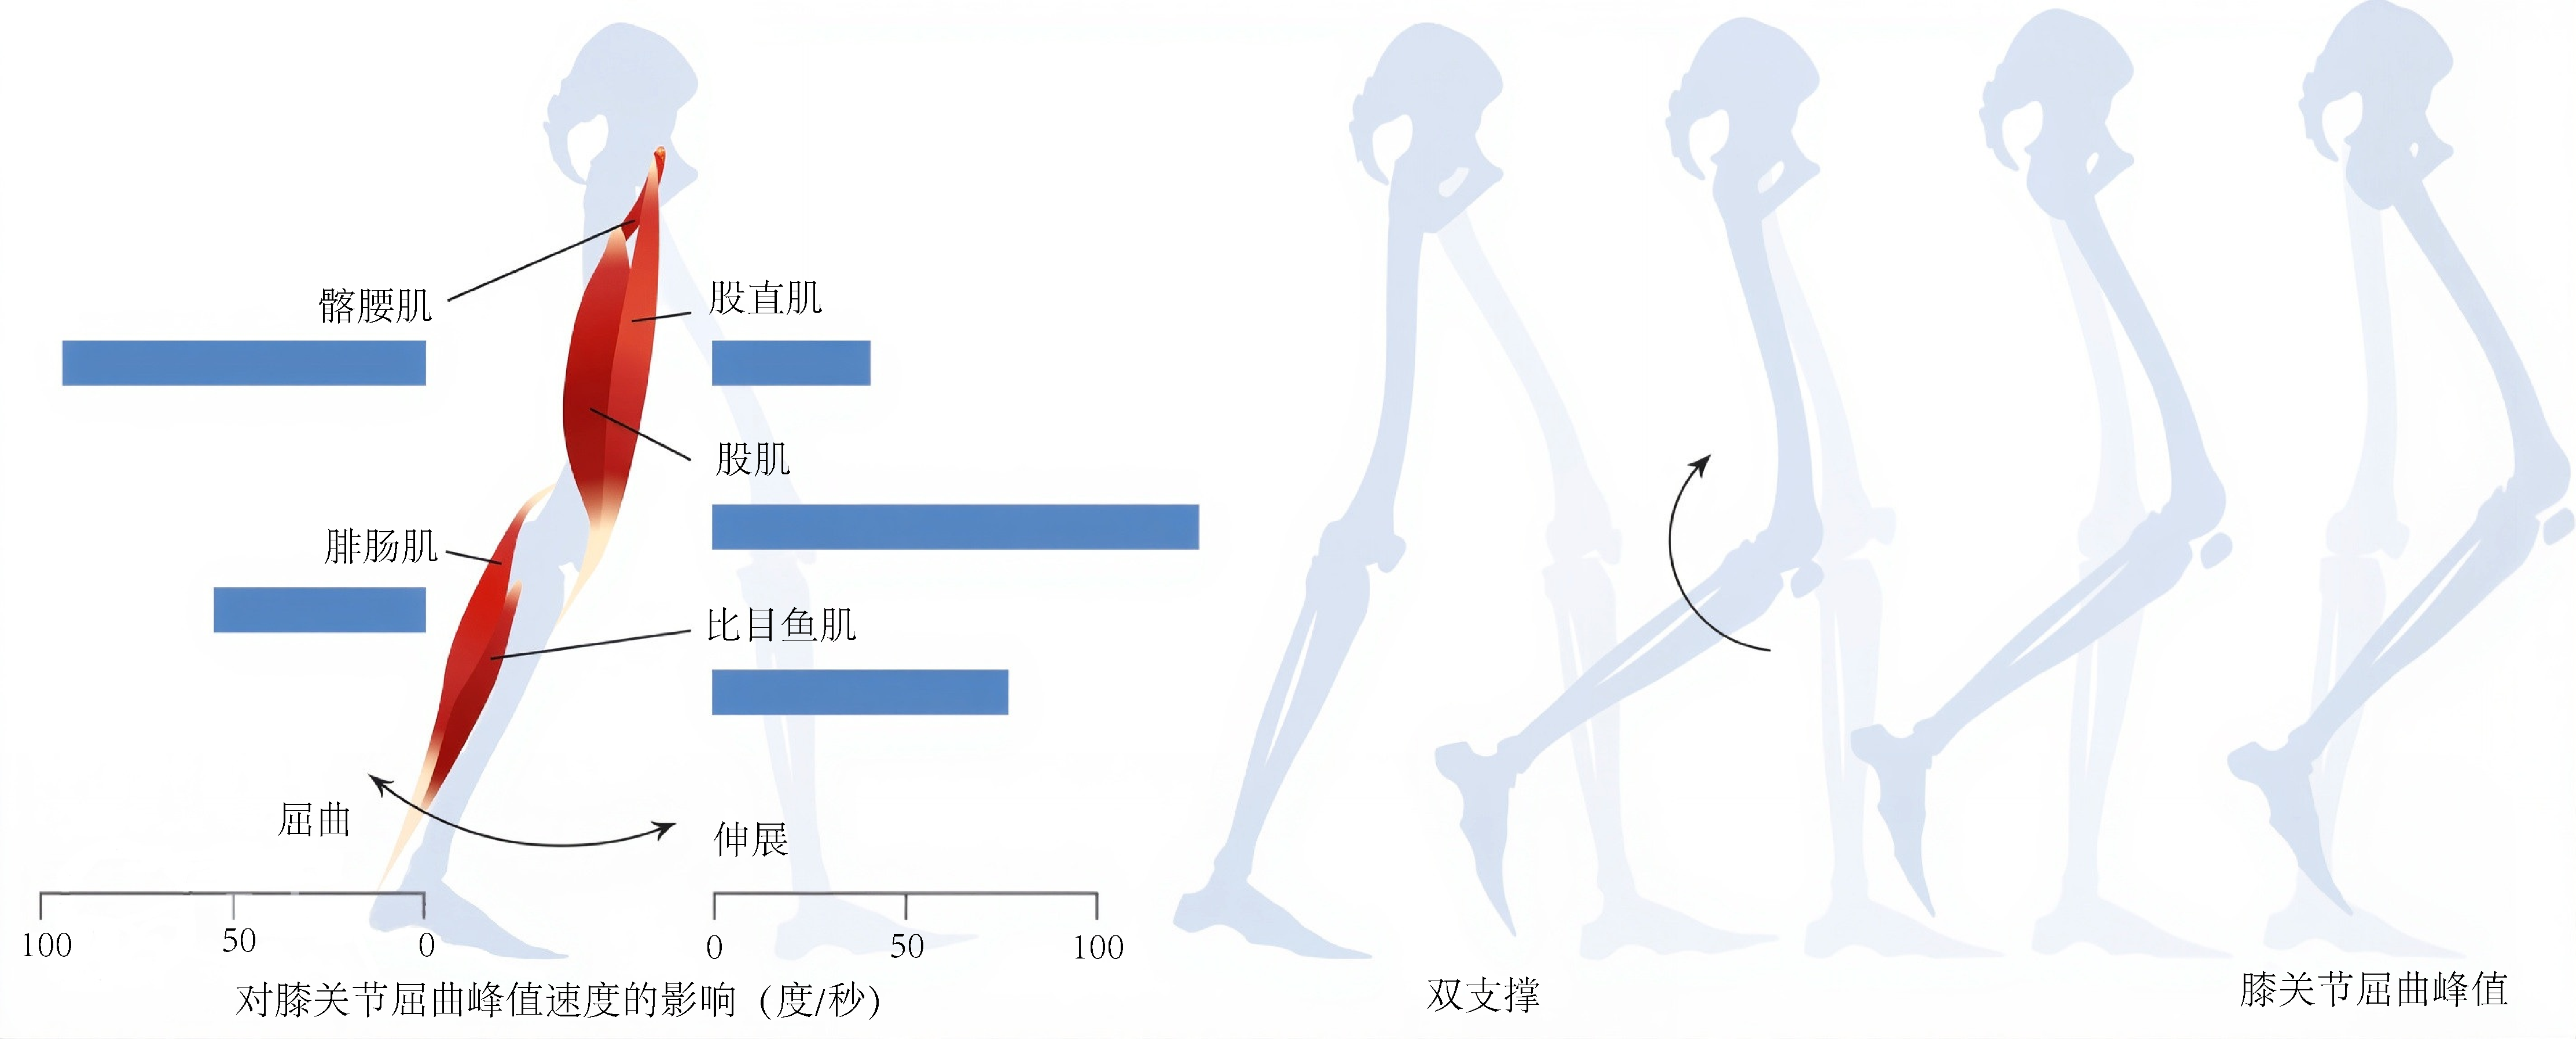
\includegraphics[width=1.0\linewidth]{chap11/11_4}
	\caption{双支撑时膝关节快速屈曲,导致足尖离地时膝关节屈曲速度较高。
		由于髂腰肌和腓肠肌产生的力量,双支撑时膝关节屈曲速度加快,而股四头肌、比目鱼肌和股直肌产生的力量则限制了屈曲速度。
		数据来自 Goldberg 等人 (2004)。 \label{fig:11_4}}
\end{figure}


挥杆动态也受挥杆过程中肌肉活动的影响。
例如,腘绳肌在挥杆期接近尾声时起着重要作用(图~\ref{fig:11_5})。
腘绳肌的动作很复杂,因为它们交叉于髋部和膝部的后方,从而产生髋部伸展力矩和膝部屈曲力矩。
膝部屈曲力矩产生膝部屈曲加速度,而髋部伸展力矩则产生几乎相等的膝部伸展加速度;
因此,腘绳肌在膝部产生的净作用很小。
Allison Arnold 对挥杆期的模拟进行了分析,结果表明腘绳肌的主要作用是产生小腿向后的加速度(Arnold 等人,2007)。
因此,腘绳肌会在挥杆结束时减慢肢体的速度。
股直肌则具有相反的作用——在挥杆开始时使肢体向前移动。


\begin{figure}[!htb]
	\centering
	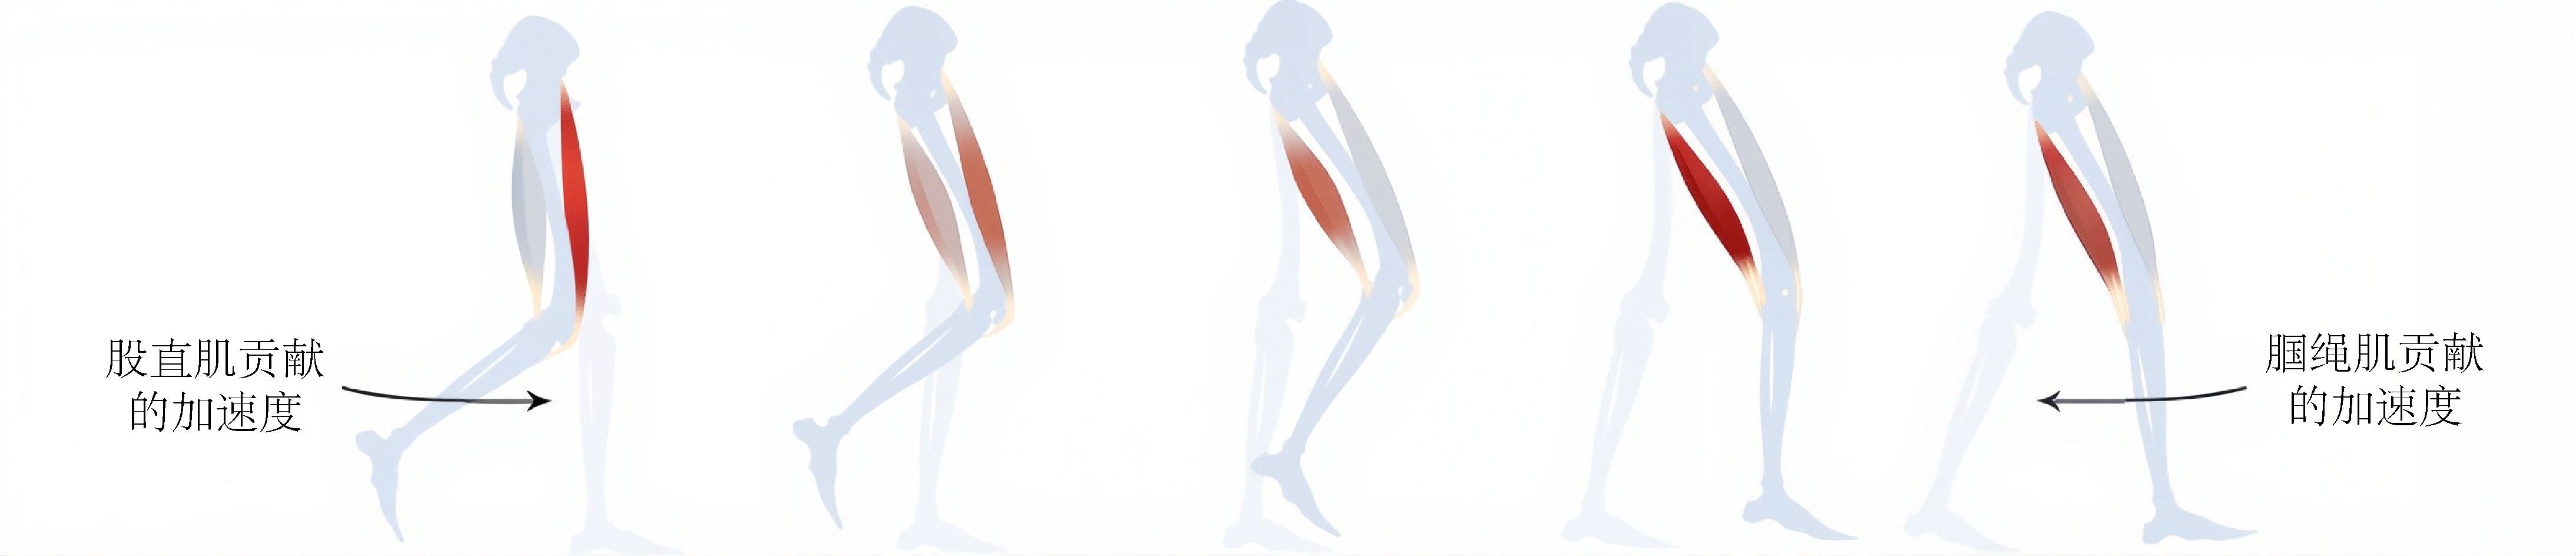
\includegraphics[width=1.0\linewidth]{chap11/11_5}
	\caption{股直肌在摆动初期活跃,加速肢体向前运动。
		腘绳肌在摆动后期活跃,在脚触地前降低摆动腿向前的速度。 \label{fig:11_5}}
\end{figure}


股直肌在摆动期调节膝关节屈曲方面也发挥着关键作用。
长期以来,人们一直认为,摆动过程中股直肌的过度活动会导致一种名为“僵膝步态”的步态异常,这种异常会导致摆动肢膝关节屈曲度降低,脚趾活动受限。
我们利用肌肉驱动模拟研究了摆动期前和摆动期股直肌过度活动对膝关节僵硬步态的影响程度。
我们将在下一节中看到这项研究的结果。


\section{膝关节僵硬步态中的肌肉动作}

膝僵硬步态的特征是摆动期膝关节屈曲峰值减弱和延迟(图 2.22),是脑瘫儿童和中风成人中最常见的步态问题之一。
摆动期膝关节屈曲不足会导致绊倒和跌倒,以及代偿运动效率低下。
尽管膝僵硬步态很普遍,但其原因尚不清楚。
多种因素可能导致膝僵硬步态,但股直肌过度活动被认为是主要原因。
常见的治疗方法是改变股直肌的功能,以改善摆动期膝关节活动。
例如,股直肌移植手术将股直肌的附着点从髌骨移至更后方的部位(例如,膝盖后方的缝匠肌),以增强膝关节屈曲。
一种非手术治疗方案是向股直肌注射肉毒杆菌毒素。
肉毒杆菌毒素是一种神经毒素,注射到肌肉中后,会阻断神经肌肉接头处乙酰胆碱的释放,从而阻止肌肉的激活。


膝关节僵硬步态的成因是什么?
股直肌的摆动相活动在导致膝关节僵硬步态方面有多重要?
这些问题固然重要,但解答起来却并非易事。
仅凭实验数据很难确定膝关节僵硬步态的成因,而且个体差异很大。
治疗结果也各不相同——有些患者术后膝关节屈曲功能得到改善,而有些则没有。
这些挑战促使我开发肌肉驱动的膝关节僵硬步态模拟系统。


我们使用了肌肉驱动的模拟来检查在摆动之前和摆动期间股直肌的活动如何影响膝关节屈曲。
Jeff Reinbolt 创建的模拟重现了膝关节僵硬步态患者的动态。
为了研究股直肌活动对膝关节运动的影响,Jeff 在模拟中消除了股直肌的刺激,首先在摆动之前,然后在摆动期早期(图~\ref{fig:11_6})。
我们发现在两种情况下膝关节屈曲都有所增加,但在摆动之前(“摆动前”)消除股直肌活动时,膝关节屈曲的增加幅度更大。
这表明,股直肌在摆动前的活动可能是限制许多膝关节僵硬步态患者膝关节屈曲的原因,而不是通常认为的摆动期间的活动。


\begin{figure}[!htb]
	\centering
	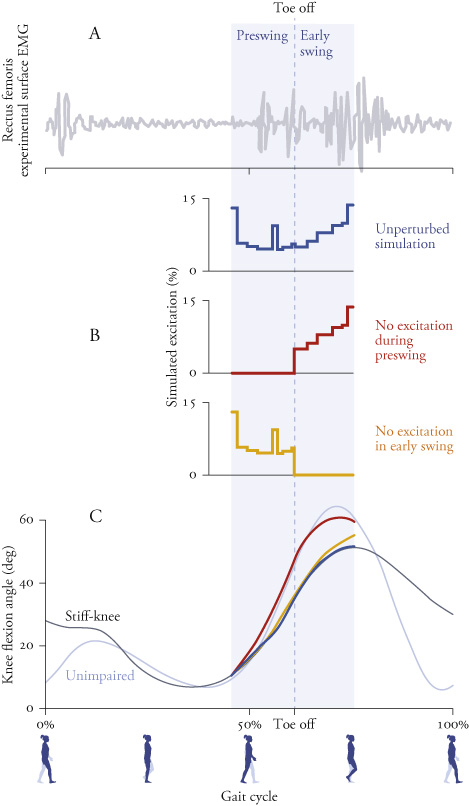
\includegraphics[width=0.75\linewidth]{chap11/11_6}
	\caption{用于比较在摆动前和摆动初期消除股直肌活动时膝关节屈曲峰值增加情况的方法。
		(A)膝关节僵硬受试者一个步态周期内的股直肌肌电图。
		(B)在摆动前(红线)和摆动初期(橙线)消除股直肌刺激。
		(C)在摆动前(红线)消除股直肌活动时,模拟的膝关节屈曲角度变化比摆动初期(橙线)更大。
		改编自 Reinbolt 等人 (2008)。 \label{fig:11_6}}
\end{figure}


这个例子说明了肌肉功能的一个重要特征——肌肉的活动会影响未来的运动。
正如我们所见,肌肉兴奋和肌肉力量产生之间存在延迟,肌肉力量产生和关节位置明显变化之间也存在延迟。
因此,在尝试识别哪些肌肉产生了异常运动时,我们必须考虑运动之前的肌肉活动。
在关注事件期间或之后发生的肌肉活动(例如,在膝关节屈曲达到峰值的瞬间)可能要等到肌肉力量产生一段时间后才会对个体的运动产生影响。
这句话可能看起来很明显,但在尝试确定哪些肌肉导致异常运动时,它常常被忘记。
我参加过很多会议,都有专家提出,异常运动后发生的异常肌电图导致了该运动。
事情根本不可能这样发生。


我的研究小组还使用了肌肉驱动的膝关节僵硬步态模拟,以研究股直肌移植手术改变肌肉功能的机制。
Melanie Fox 在计算机模型中改变了股直肌,以模拟各种治疗的效果(图~\ref{fig:11_7})。
模拟结果显示,在将股直肌模拟移植至缝匠肌后,膝关节屈曲峰值改善最大,该手术将股直肌从膝关节伸展力矩的产生器转变为膝关节屈曲力矩的产生器。将股直肌移植至髂胫束后,膝关节屈曲峰值改善较小。
模拟肉毒杆菌毒素注射到股直肌中,消除了其产生的膝关节伸展力矩和髋关节屈曲力矩,其改善效果比任何一种模拟移植都要小。
这些模拟表明,股直肌移植改善膝关节屈曲的主要机制是减少肌肉的膝关节伸展力矩。
改善的次要机制是保持肌肉的髋屈曲力矩,从而引起膝屈曲。


\begin{figure}[!htb]
	\centering
	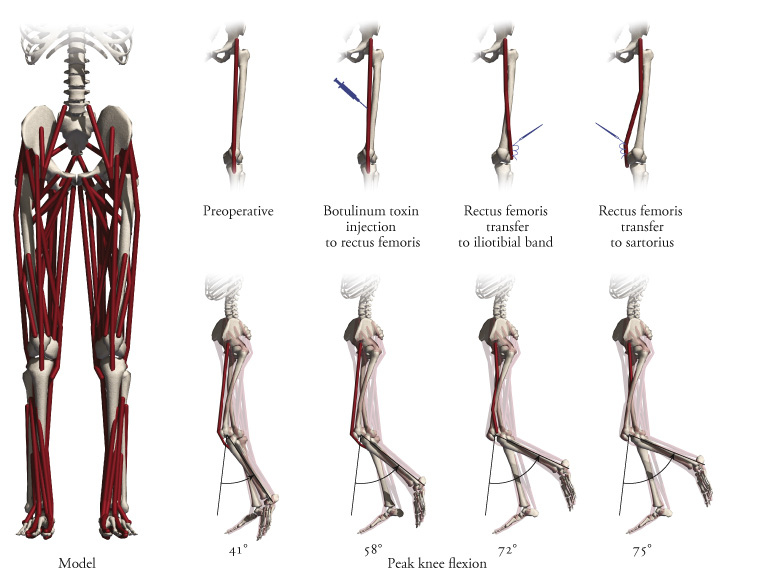
\includegraphics[width=1.0\linewidth]{chap11/11_7}
	\caption{针对一名膝关节僵硬步态患者,在模拟术前步态和三种候选干预措施后的步态时,下肢模型的膝关节屈曲峰值(左)。
		改编自 Fox 等人 (2009)。 \label{fig:11_7}}
\end{figure}


接下来,我们研究了脑瘫患者接受股直肌移植手术后,足尖离地时膝关节屈曲速度、双支撑时关节力矩与僵硬步态改善之间的关系。
僵硬步态的受试者往往在足尖离地时表现出异常低的膝关节屈曲速度,并在双支撑时表现出过大的膝关节伸展力矩。
术后恢复良好的受试者,这些指标在术后有显著改善;
而术后恢复不良的受试者则没有。
因此,虽然在摆动期观察到僵硬步态,但其主要原因是站立后期肌肉活动异常。
正如卡尔$\cdot$萨根曾经说过的:“你必须了解过去,才能理解现在。”


\section{不同步行速度下的肌肉动作}

我们在第~\ref{chap:chap2}~章中了解了步行速度如何影响关节运动学和地面反作用力。
肌肉激活度也会随着步行速度而变化,这不足为奇。
图~\ref{fig:11_8}~显示了四种速度下行走时主要下肢肌肉的激活模式。
为了获得这些模式,Edith Arnold 测量了健康受试者在跑步机上行走时的表面肌电图 (EMG) 信号。
然后,对 EMG 信号进行 30 Hz 高通滤波、整流,再进行 10 Hz 低通滤波(图 4.14)。
每位受试者滤波后的 EMG 测量值均通过一系列活动(包括步行、跑步和最大自主收缩)中检测到的每块肌肉的最大 EMG 值进行归一化(即,归一化后,最大活动量 = 1)。


\begin{figure}[!htb]
	\centering
	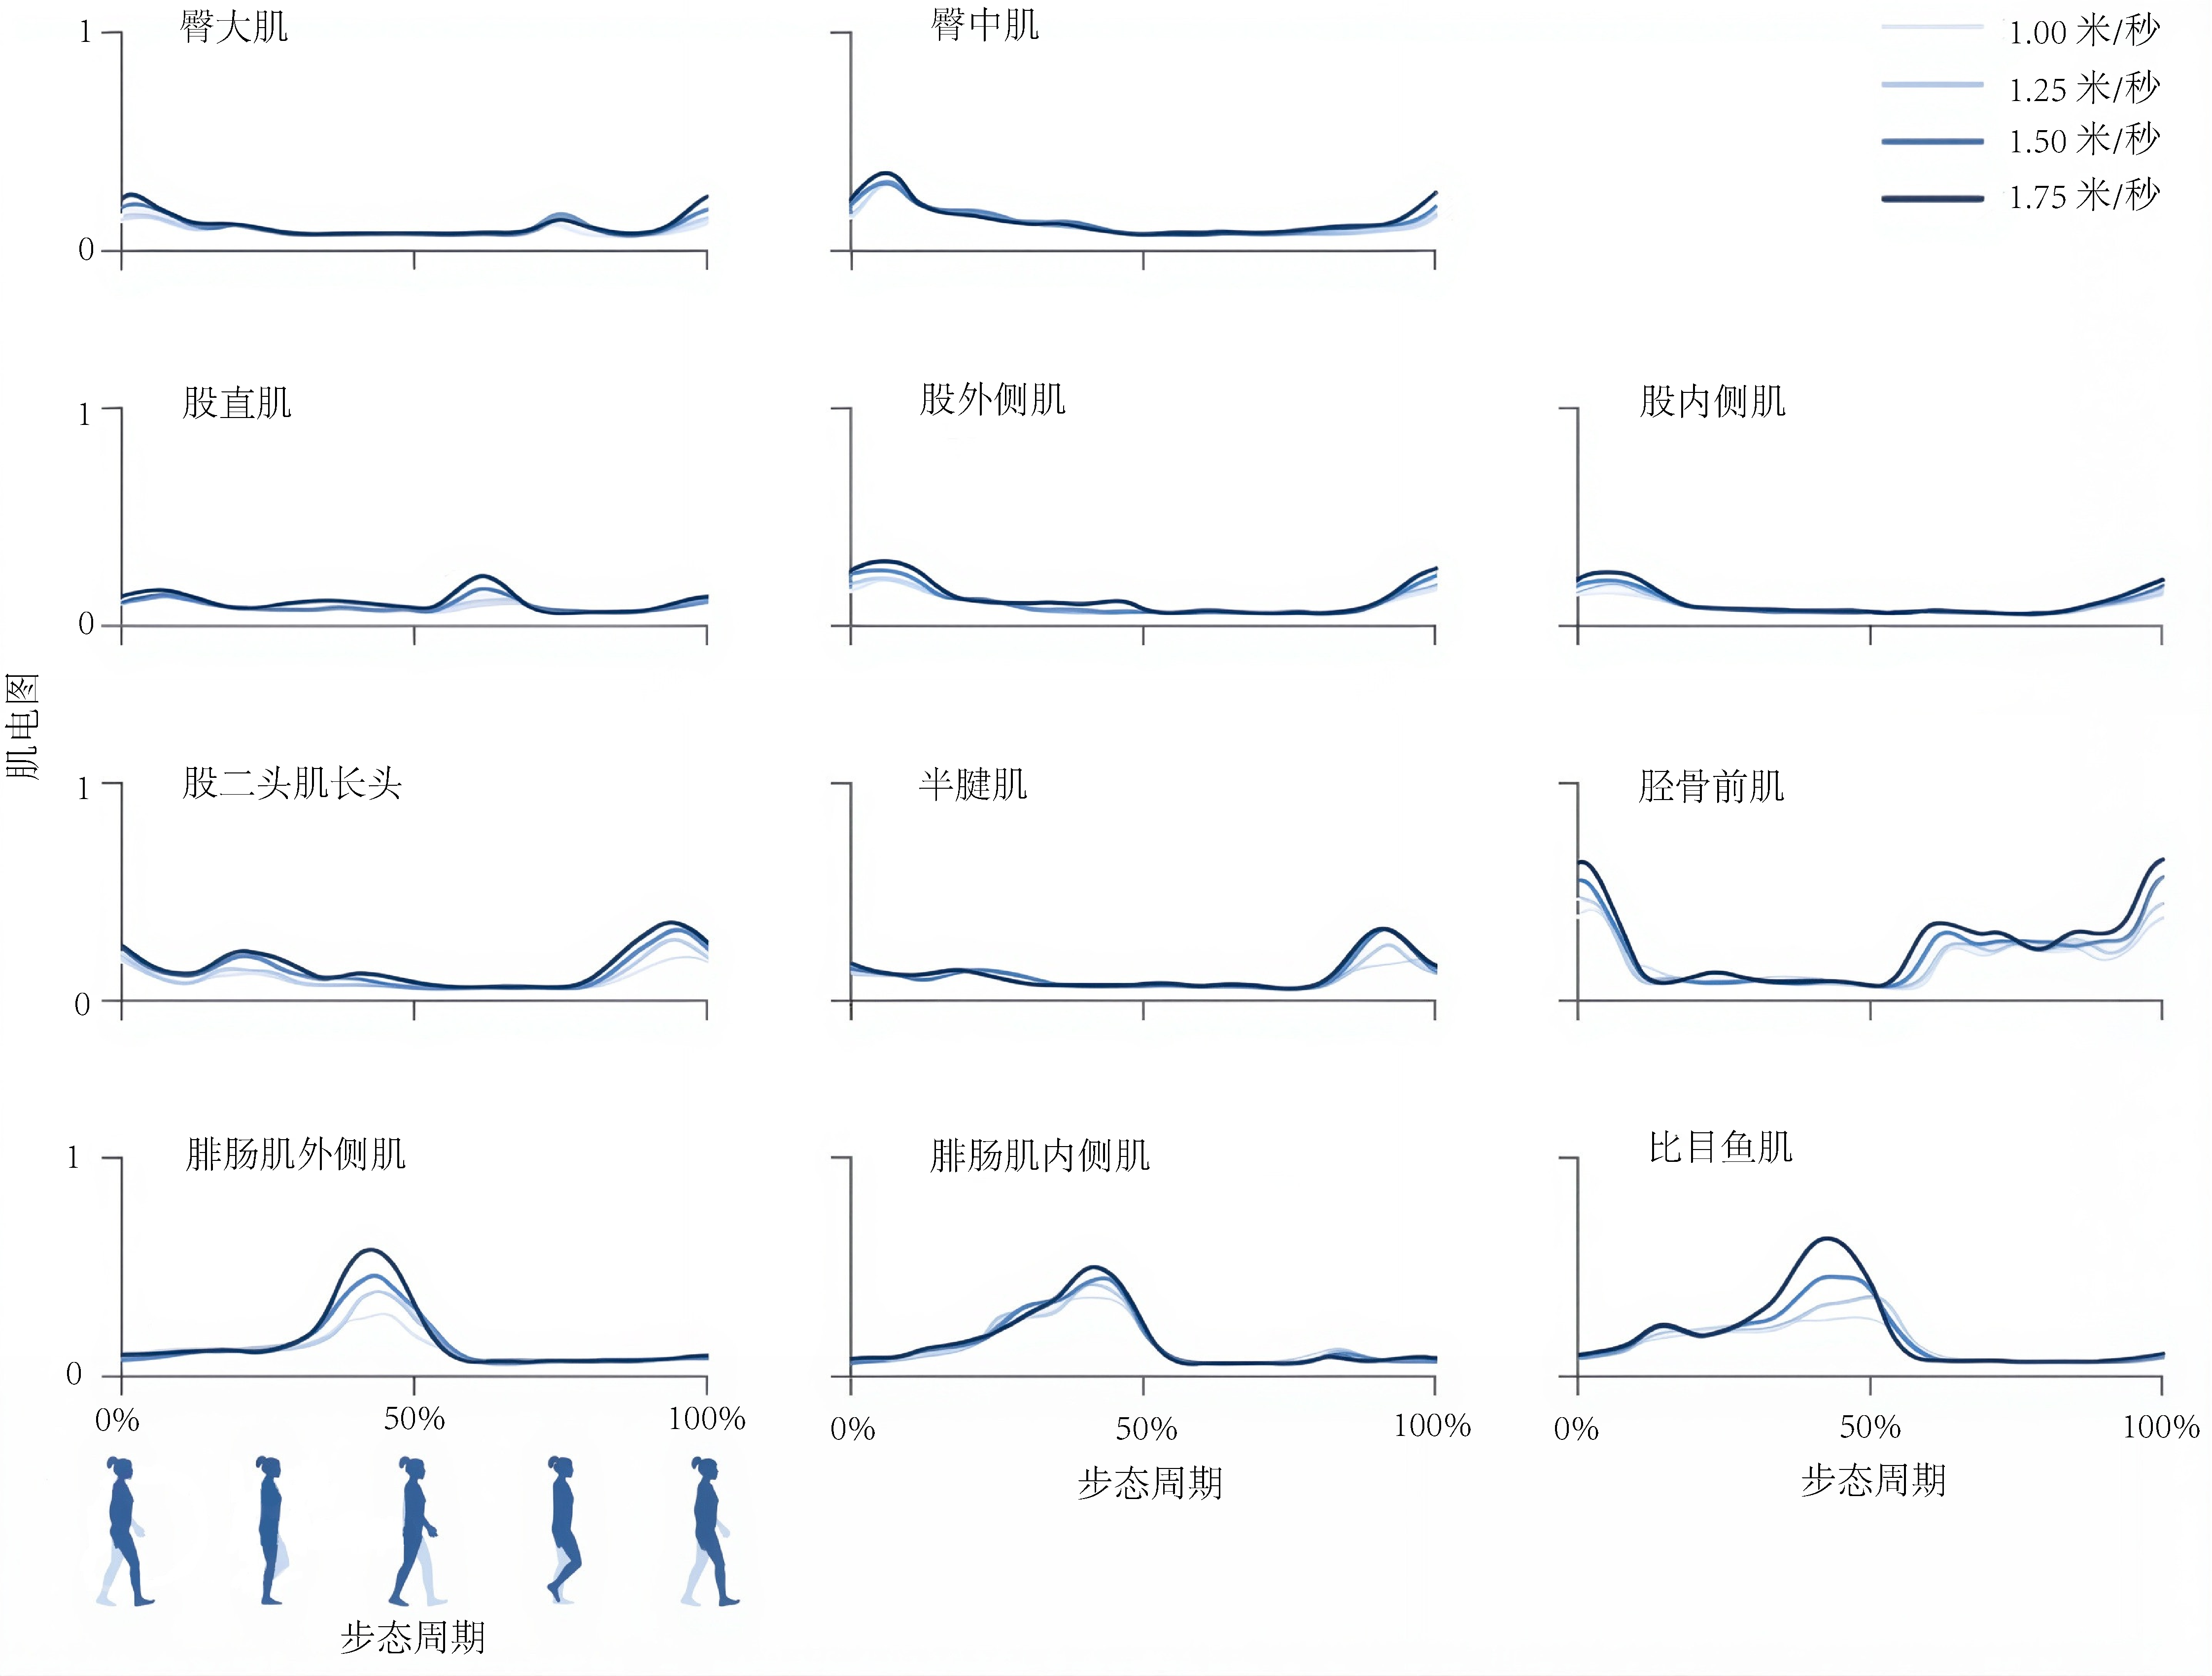
\includegraphics[width=1.0\linewidth]{chap11/11_8}
	\caption{四种步行速度(1.00 至 1.75 米/秒)下测量的 11 块肌肉的平均标准化肌电图模式。
		原始肌电图信号经过校正、滤波和标准化,取各块肌肉在各种活动中检测到的最大值。
		数据来自 Arnold 等人(2013 年)。 \label{fig:11_8}}
\end{figure}


在典型的步行过程中,我们观察到臀大肌、臀中肌、股外侧肌和股内侧肌在站立初期的激活,所有这些肌肉都对地面反作用力做出重要贡献。
我们还看到胫骨前肌在站立初期的强烈活动。在典型的步态中,胫骨前肌在拉长的同时产生力量,充当制动器以控制脚部向地面的下沉(图~\ref{fig:11_9});
如果胫骨前肌疲劳或麻痹,则可能出现“脚拍”。
在剧烈徒步后的第二天,您可能感到小腿酸痛;这是由于胫骨前肌在充当制动器时受到的拉伤。
胫骨前肌在摆动时也会活跃,以抬起脚趾并避免绊倒。
一般而言,肌肉活动随着步行速度的增加而增加(图~\ref{fig:11_8})。
在站立后期,腓肠肌和比目鱼肌的活跃度会随着重心前移而增强(图~\ref{fig:11_2})。
股直肌在摆动期开始时激活度最高,而腘绳肌(包括股二头肌长头和半腱肌)在摆动期结束时激活度最高。


\begin{figure}[!htb]
	\centering
	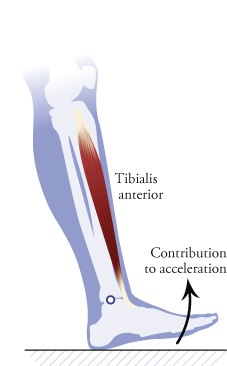
\includegraphics[width=0.4\linewidth]{chap11/11_9}
	\caption{胫骨前肌在脚跟着地时活跃,并产生力量来控制站立初期脚部向地面的下降。 \label{fig:11_9}}
\end{figure}


许多患有神经肌肉障碍的人走路很慢。评估患者的步态需要我们区分病理引起的偏差和仅仅由于缓慢行走引起的变化。
在这里,我们研究肌肉如何在不同的步行速度下调节地面反作用力。
我的研究小组与吉列儿童专科医疗保健的生物工程师 Michael Schwartz 合作,分析了由肌肉驱动的三维步行模拟。
我们使用 OpenSim 重现了 8 名健康个体以四种速度行走的运动:非常慢、慢、自然和快速(图~\ref{fig:11_10})。
这些速度类别是根据无量纲步行速度定义的:“快速”包括比每个人的平均“自然”步行速度至少快一个标准差的步行试验,“慢速”试验比自然速度慢一到三个标准差,“非常慢”试验比自然速度慢三个以上标准差。

\begin{figure}[!htb]
	\centering
	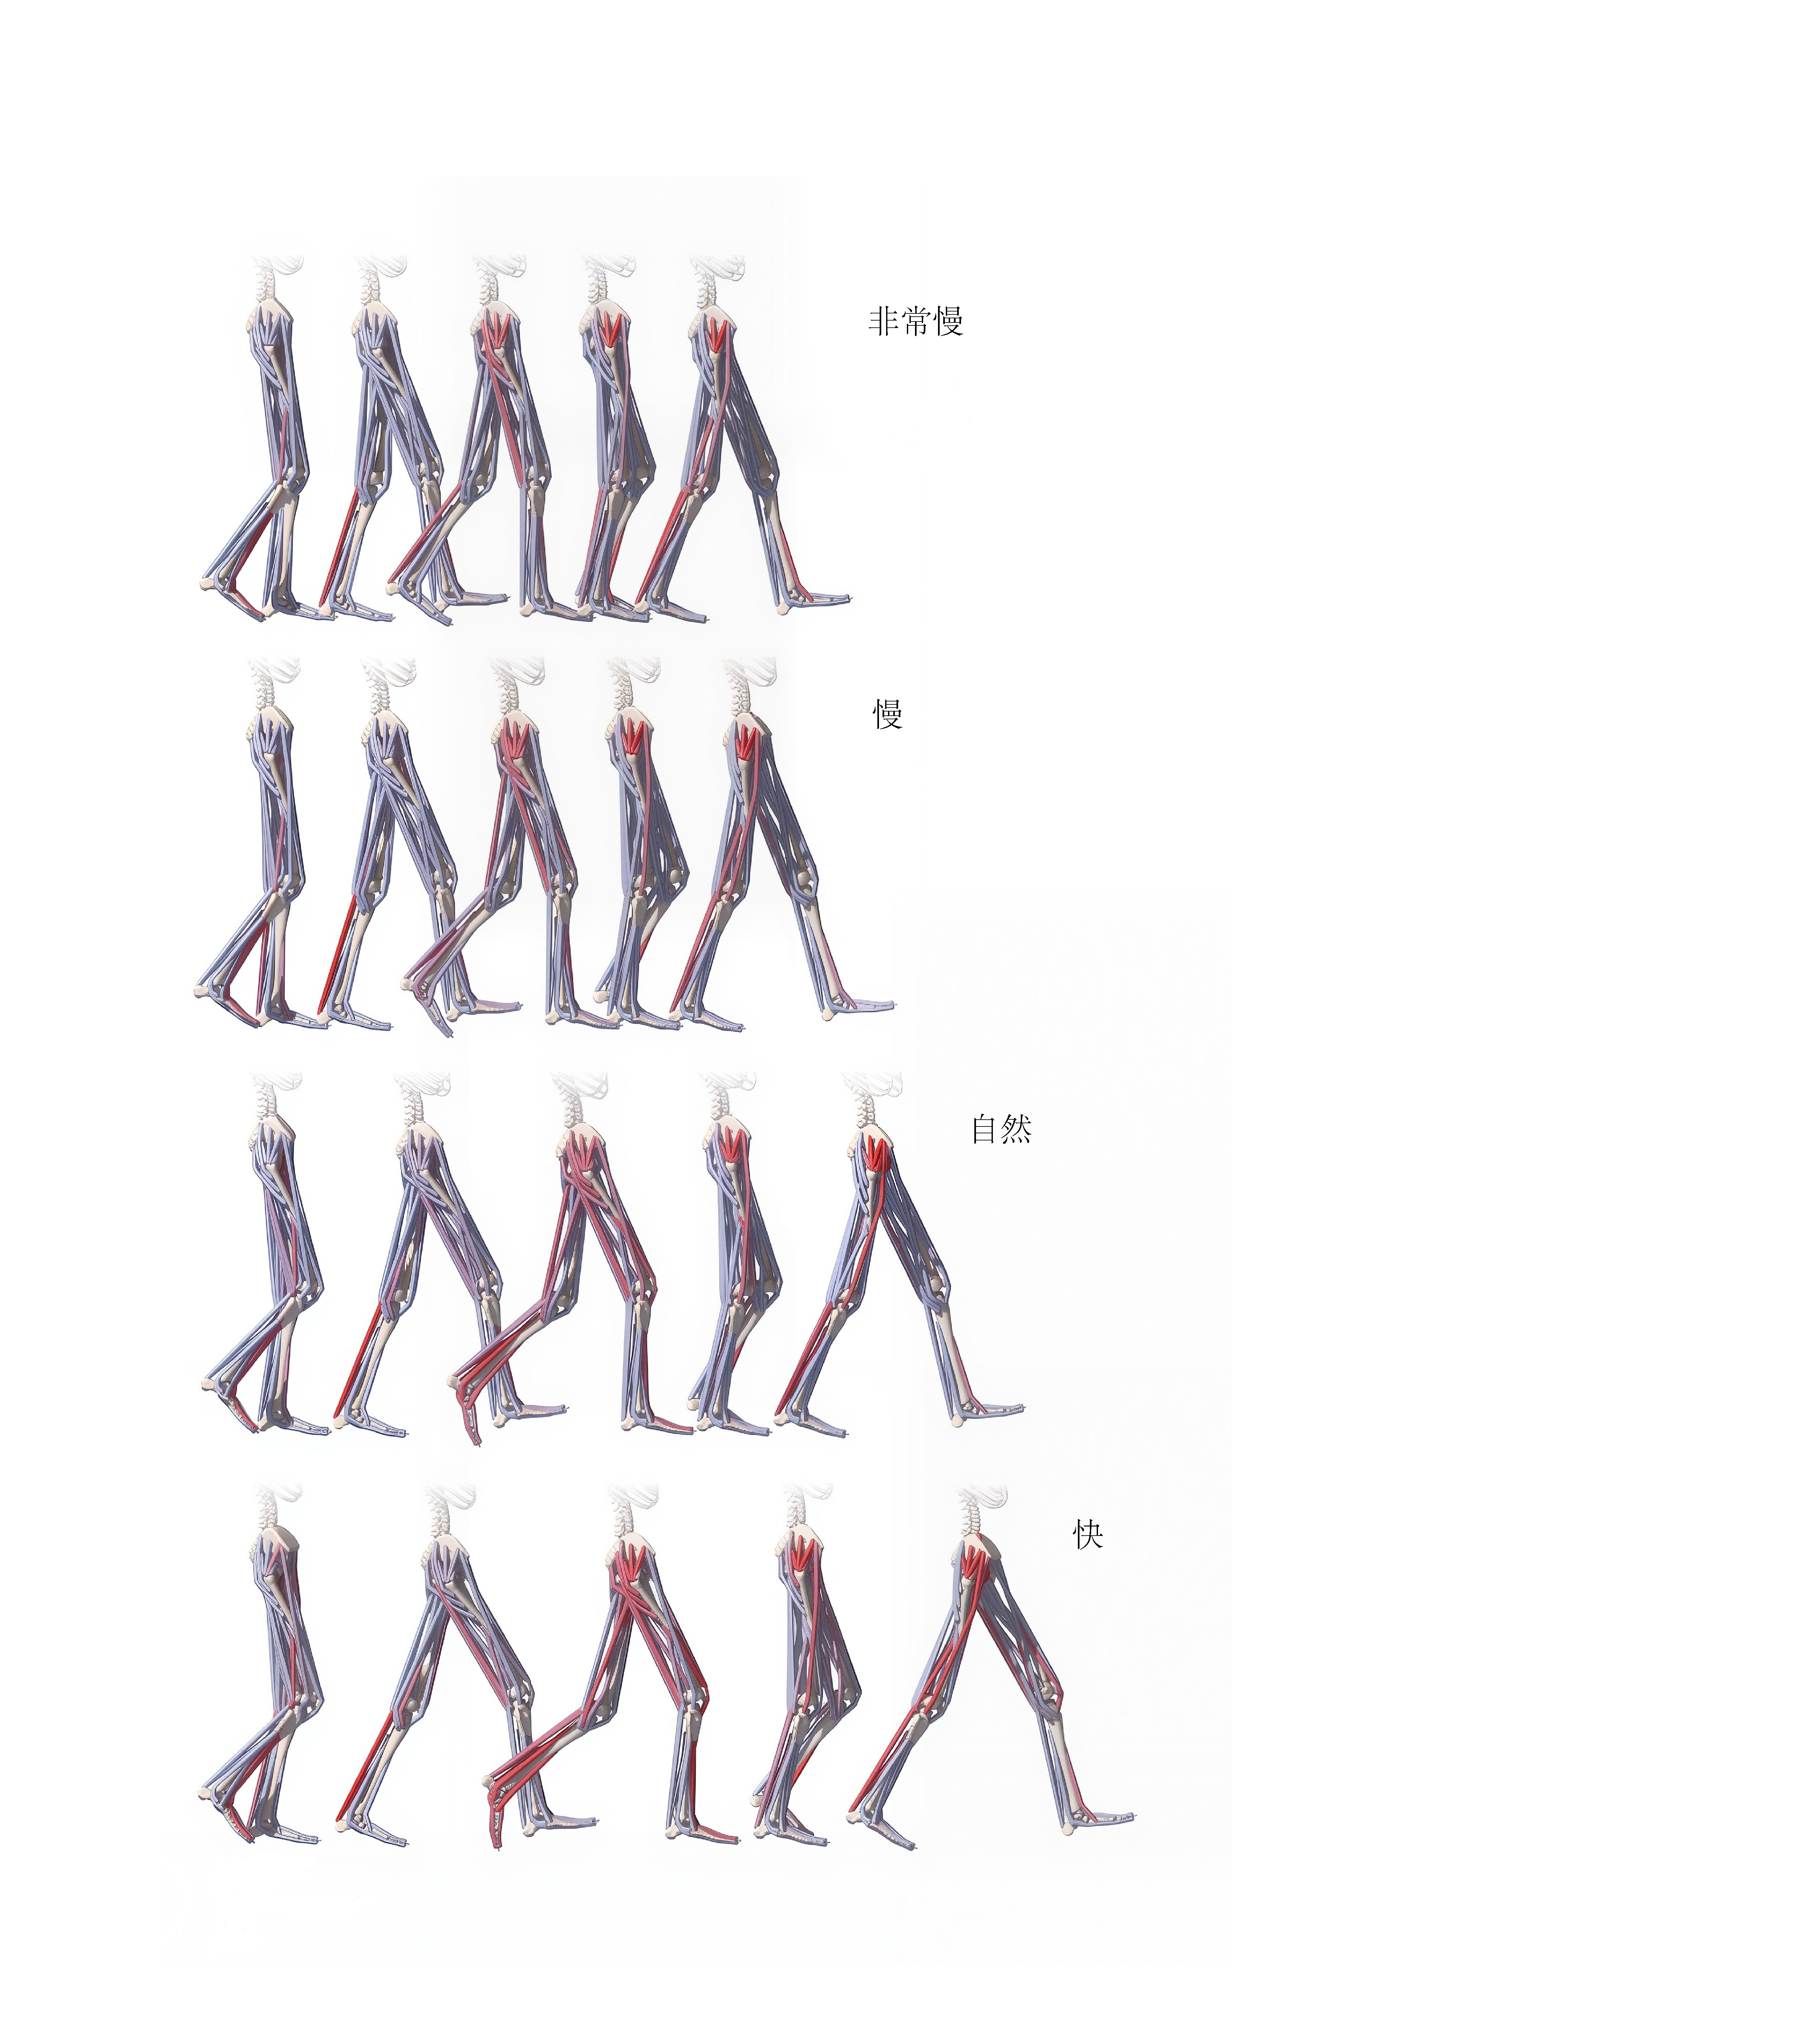
\includegraphics[width=1.0\linewidth]{chap11/11_10}
	\caption{代表性受试者以四种速度行走的肌肉驱动模拟可视化。
		肌肉颜色表示模拟激活程度,从无激活(蓝色)到完全激活(红色)。
		数据来自 Liu 等人(2008)。 \label{fig:11_10}}
\end{figure}


我们发现,肌肉对支撑和推进的贡献会随着步行速度的增加而增加,尤其是在低速和自然速度步行之间的差异显著增加(图~\ref{fig:11_11})。
在极慢速和慢速步行过程中,早期站立时较直的肢体(而非肌肉)提供了大部分对抗重力的支撑。


\begin{figure}[!htb]
	\centering
	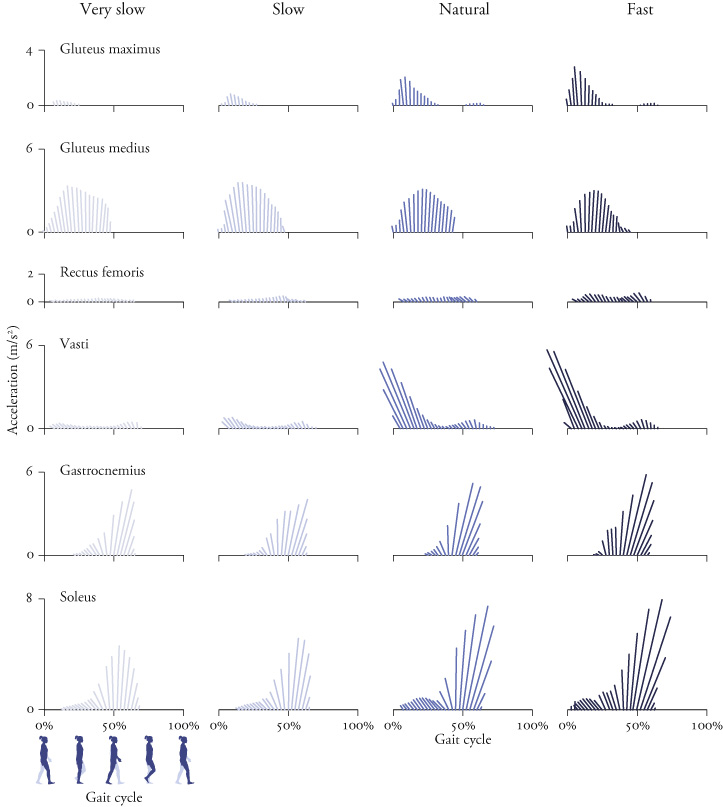
\includegraphics[width=1.0\linewidth]{chap11/11_11}
	\caption{代表性受试者以四种速度行走的肌肉驱动模拟可视化。
		肌肉颜色表示模拟激活程度,从无激活(蓝色)到完全激活(红色)。
		数据来自 Liu 等人(2008)。 \label{fig:11_11}}
\end{figure}

这些结果凸显了简单动态步行模型和肌肉驱动动态步行模型之间的相似之处。
例如,在肌肉驱动模拟中,我们观察到双支撑过程中后肢肌肉向前加速(推进),前肢肌肉向后加速(制动),这与简单模型中重心速度的重定向一致。
Max Donelan 及其同事(2002)使用了一个具有刚性肢体的简单模型来证明施加于后肢的力会重定向重心的速度;
肌肉驱动的步行模拟表明腓肠肌和比目鱼肌发挥了这一作用。
在简单模型中,类似支柱的前肢的制动作用源于地面反作用力被动传递到重心(Kuo,2002)。
同样,在我们最慢的步行模拟中,我们观察到骨骼排列发挥了类似支柱的功能。


简单模型和肌肉驱动模型之间的差异在更快的步行速度下更加明显。
随着步行速度的增加,站立初期和后期前后地面反作用力的大小也会增加(图2.20),从而产生更大的制动力和推进力。
肌肉驱动模拟表明,腓肠肌和比目鱼肌从后肢提供了所需的更大推进力。
然而,由于膝关节屈曲,在更快的步行速度下,前肢不再像支柱一样,无法被动地传递地面反作用力。
人类的膝关节屈曲需要股四头肌的主动调节,股四头肌从前肢提供制动力。


\section{蹲伏步态中的肌肉动作}

许多脑瘫患者行走时呈蹲伏步态,即膝盖和臀部过度屈曲。
蹲伏步态会导致膝盖疼痛并增加能量消耗。
了解蹲伏步态过程中肌肉如何加速重心移动,有助于深入了解这种疾病的生物力学原理,并提出改善步行的方法。


肌肉驱动模拟揭示了肌肉对重心垂直和前后加速度的贡献在蹲伏步态和典型步态中有何不同,以及这些肌肉贡献如何随蹲伏程度的变化而变化。
为了计算肌肉对身体重心加速度的贡献,Kat Steele 分析了正常发育儿童和不同蹲伏程度的脑瘫儿童的三维步行模拟(图~\ref{fig:11_12})。


\begin{figure}[!htb]
	\centering
	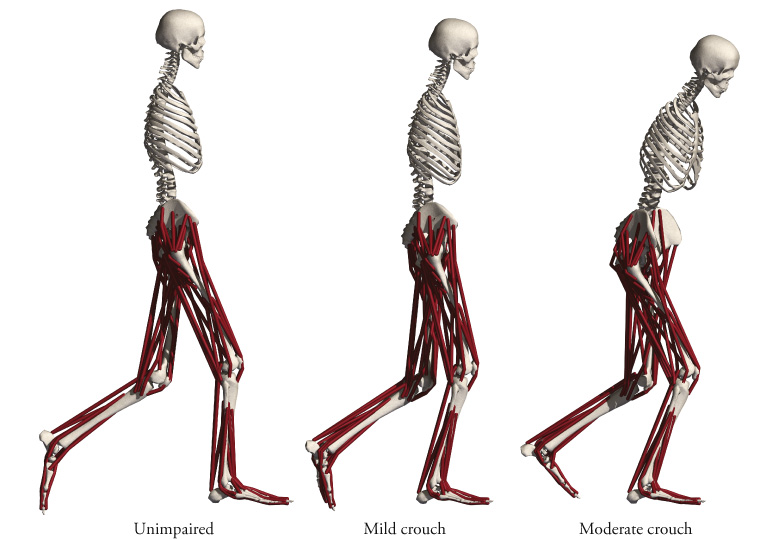
\includegraphics[width=1.0\linewidth]{chap11/11_12}
	\caption{用于创建肌肉驱动模拟的肌肉骨骼模型,分别针对具有典型步态的个体(左)以及以轻度和中度蹲伏步态行走的脑瘫个体(中和右)。
		改编自 Steele 等人 (2013)。 \label{fig:11_12}}
\end{figure}


模拟显示,与未受损步态一样,两组肌肉主要负责在蹲伏步态中加速重心向上并调节前后加速度:股四头肌和踝跖屈肌。
然而,与典型步态不同,这些肌肉在整个站立姿势中加速重心,并引起较大的、相反的前后加速度。
在蹲伏步态中,踝跖屈肌在整个站立姿势中加速重心向上和向前,而股四头肌使重心向上和向后加速(图~\ref{fig:11_13})。
在未受损步态下,股四头肌和跖屈肌活动的适当协调提供了一种有效的步行策略。这种策略在蹲伏步态期间受到影响,需要这些肌肉对垂直和前后加速度做出更持续的贡献。这就像踩着刹车开车(图~\ref{fig:11_14})。


\begin{figure}[!htb]
	\centering
	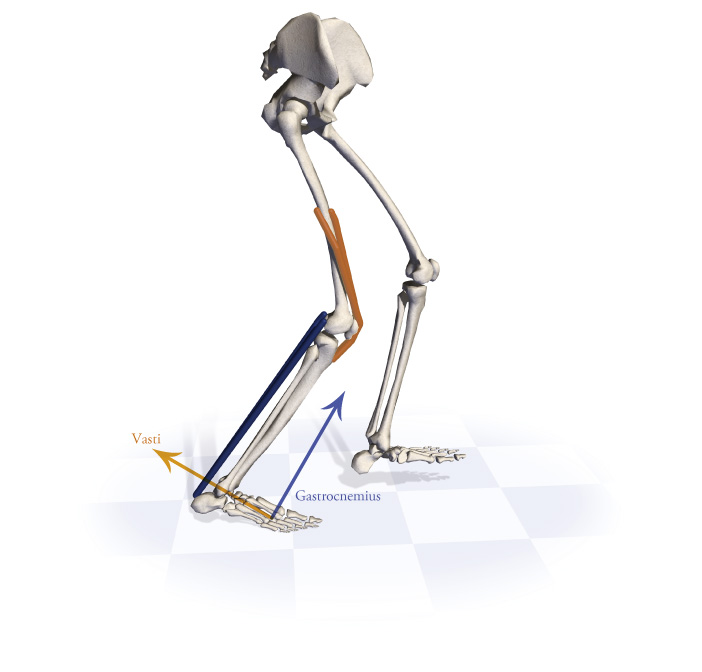
\includegraphics[width=1.0\linewidth]{chap11/11_13}
	\caption{在蹲伏步态期间,股肌和跖屈肌在整个站立过程中都处于活跃状态,并产生持续向上的地面反作用力来支撑身体重量,但这些肌肉群也会向前和向后产生相反的地面反作用力。 \label{fig:11_13}}
\end{figure}


\begin{figure}[!htb]
	\centering
	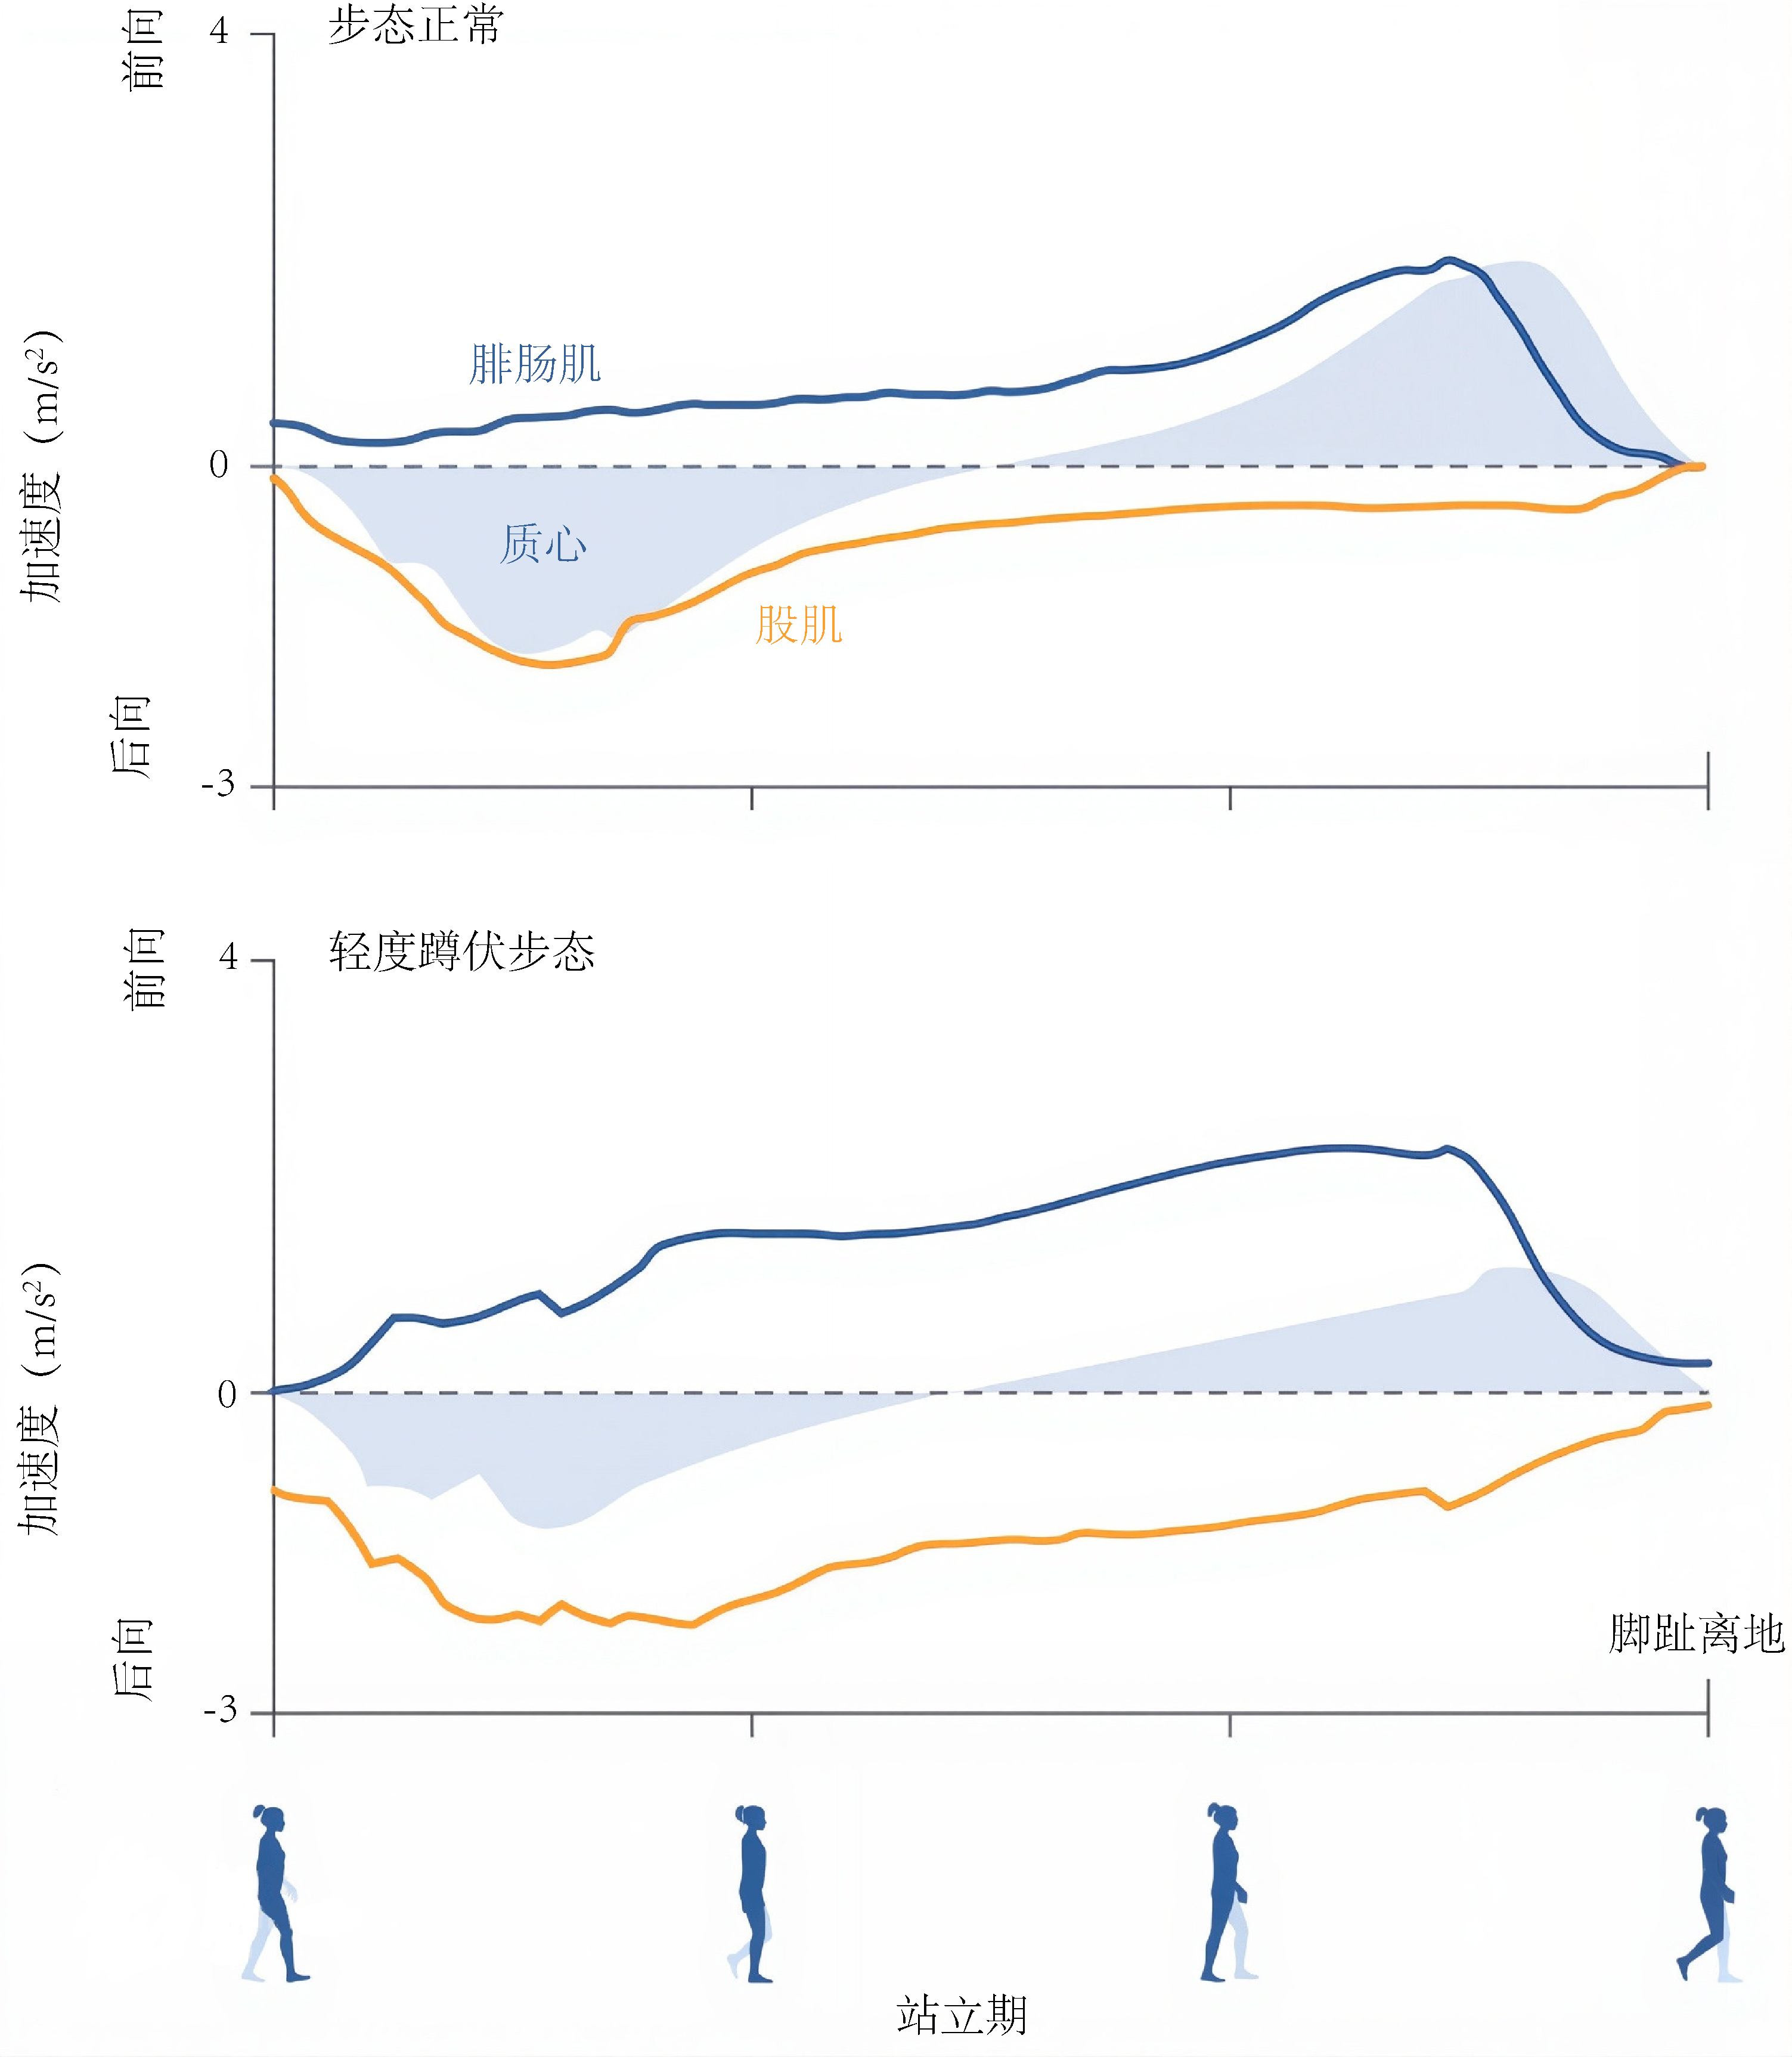
\includegraphics[width=0.9\linewidth]{chap11/11_14}
	\caption{站立时腓肠肌和股四头肌产生的重心前后加速度。
		蓝色阴影区域表示实验测量的重心加速度(即前后地面反作用力除以身体质量)。
		数据来自 Steele 等人(2013)。 \label{fig:11_14}}
\end{figure}


在未受损步态的直立姿势下,骨骼排列支撑的体重比蹲伏姿势下更大。
因此,蹲伏步态中支撑体重的肌肉会产生更大的力量,导致蹲伏步态行走效率低下。
例如,股四头肌产生的力量在蹲伏步态中明显大于未受损步态,并且这些肌肉力量会随着蹲伏程度的增加而增加(图~\ref{fig:11_15})。
我们的模拟表明,蹲伏程度的增加也会导致膝关节负荷增加,这可能会磨损膝关节并引起疼痛。


\begin{figure}[!htb]
	\centering
	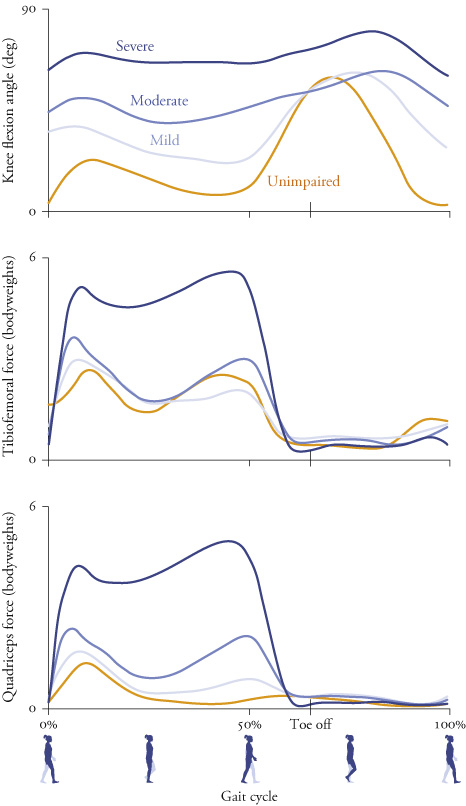
\includegraphics[width=0.8\linewidth]{chap11/11_15}
	\caption{受试者在一个步态周期内,以正常步态行走,以及轻度、中度和重度蹲伏步态行走,其平均膝关节屈曲角度(上)、膝关节压缩力(中)和股四头肌力量(下)。
		数据来自 Steele 等人 (2012)。 \label{fig:11_15}}
\end{figure}


我们的模拟还表明,由于骨骼支撑减少,蹲伏姿势会增加肌肉加速重心向上运动的需求。
在蹲伏步态中,股四头肌和踝跖屈肌产生最大的重心向上加速度,但臀中肌加速重心向上运动的能力在蹲伏步态中会受到影响。
在未受损的步态中,臀中肌在从股四头肌活动过渡到踝跖屈肌活动的过渡过程中,会在站立中期加速重心向上运动。
当以蹲伏姿势行走时,臀中肌对向上加速度的贡献会减小;
因此,股四头肌和跖屈肌的贡献必须在步态周期的更大部分时间内持续,以支撑站立中期的重心(图~\ref{fig:11_14})。


以上结果为治疗方案提供了有益的指导。
蹲伏行走时,股大肌和股直肌的负荷更大,这可能导致疲劳。
力量训练或其他提高这些肌肉耐力的项目可能有助于减轻蹲伏步态患者的疲劳。
踝跖屈肌是蹲伏步态时加速重心向上和向前移动的关键肌肉,是力量训练项目的良好目标。
Jack Engsberg 及其同事(2006 年)报告称,在加强踝跖屈肌后,站立时膝关节屈曲得到改善。
通过肌腱延长手术、神经肌肉毒素注射或其他常用于脑瘫患者的手术来削弱腓肠肌或比目鱼肌,可能会降低患者支撑自身体重的能力。
踝足矫形器和辅助踝跖屈肌的主动装置可以减少膝关节屈曲,减轻膝关节负荷,并提高蹲伏步态患者的步行效率。


我们如何利用肌肉驱动模拟的洞见来改善我在本章开头介绍的那位13岁女孩的步态?
首先,我们使用肌肉骨骼模型确定她的腘绳肌长度足以支持正常行走,因此腘绳肌较短不太可能是导致她蹲伏步态的原因。
她适合接受腘绳肌延长手术,但我建议不要进行这项手术。
其次,我们仔细检查了她踝关节跖屈肌的肌力。
我们从肌肉驱动模拟中了解到,比目鱼肌对于产生重心向上的加速度至关重要。
她的跖屈肌肌力较弱,产生的踝关节力矩还不到正常步态所需踝关节力矩的一半。
她的理疗师推荐了一种轻便的弹簧式踝关节支架,这种支架可以放入她的鞋子中,并产生踝关节跖屈力矩来增强她的肌肉。
两周后,她戴着新的支架以更直立的姿势行走。无需进行任何痛苦的手术。
她的跖屈力矩更大了,更重要的是,踝关节支架让她在行走时膝盖和臀部的屈曲度更小。
她走路时仍然会轻微蹲伏,但能够站得更高,跟上朋友们的步伐。


\section{脚跟行走和脚尖行走}

脑瘫、中风和肌营养不良症患者通常会出现踝关节跖屈肌无力和紧张的情况。
肌肉挛缩(紧张)会导致受影响肌肉的被动僵硬程度更高。
由于骨骼畸形和神经功能缺损等并发疾病,确定这些肌肉缺陷与观察到的步态病变(例如足跟行走和足尖行走)之间的因果关系变得复杂。
Carmichael Ong 使用肌肉驱动的模拟来预测跖屈肌无力和挛缩引起的步态适应性变化,且不考虑其他缺陷。
Carmichael 开发了一个具有 9 个自由度(骨盆在矢状面上的旋转和平移,以及每条腿的髋部、膝盖和踝部屈曲)的平面模型,每条腿有 9 个肌肉肌腱执行器,代表下肢的主要肌肉群。他使用动态优化(见图9.15)来寻找肌肉协调策略,以最大限度地降低运输成本,同时避免跌倒和受伤。
使用未受损模型进行优化,产生的步态能够重现运动学、动力学和能量消耗的实验测量值。
在验证了模拟框架后,他使用存在跖屈肌无力和挛缩的模型重复了优化程序——假设这些肌肉缺陷不会影响人们以最低运输成本行走的意愿。
无力通过降低比目鱼肌和腓肠肌的最大等长力量来建模;挛缩则通过减少其最佳纤维长度来建模。


优化器在所有情况下都能产生稳定的步态,无论肌肉缺陷如何。
也就是说,每个模型都能够“学习”如何行走。
跖屈肌无力降低了模型产生踝关节跖屈力矩的能力,而踝关节跖屈力矩对于在行走过程中产生向前的推进力至关重要(图~\ref{fig:11_2})。
因此,肌力减弱的模型比未受损的模型走得慢,这种现象在跖屈肌无力的患者中也有观察到。
此外,跖屈肌无力导致模型采用“脚跟着地”或跟骨步态,着地时踝关节背屈幅度明显增大(图~\ref{fig:11_16}),这在一些跖屈肌无力但灵活的患者中也有观察到。
相比之下,跖屈肌挛缩导致“足尖行走”或马蹄足步态,模型在脚接触地时用脚趾着地,并在整个站立过程中保持脚趾着地。
严重的跖屈肌挛缩也会导致蹲伏步态。


\begin{figure}[!htb]
	\centering
	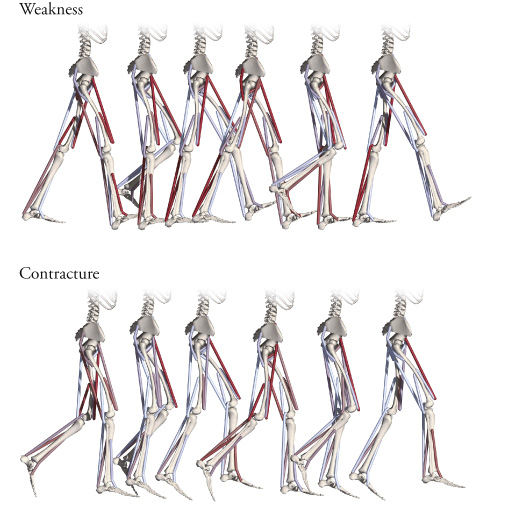
\includegraphics[width=0.8\linewidth]{chap11/11_16}
	\caption{通过最小化运输成本的动态优化,可以预测跖屈肌力量较弱时的跟腱步态(上图)以及跖屈肌挛缩时的马蹄足步态(下图)\cite{ong2019predicting}。 \label{fig:11_16}}
\end{figure}


像这样的模拟研究有助于阐明因果关系,而这些因果关系在实验研究中很难与其他因素区分开来。
这一点至关重要,因为外科手术干预基于因果推理。
如果我们不知道患者蹲伏步态的原因,或者评估错误,我们可能会让患者接受不必要且无效的手术。


\section{设备辅助行走}

外骨骼装置可以增强人体的功能。
一些最早的外骨骼类装置诞生于19世纪后期,用于辅助行走、跑步和跳跃(图~\ref{fig:11_17}),但直到最近才真正投入实用。
我们可以利用肌肉驱动的模拟来改进这些装置,并指导新技术的设计。


\begin{figure}[!htb]
	\centering
	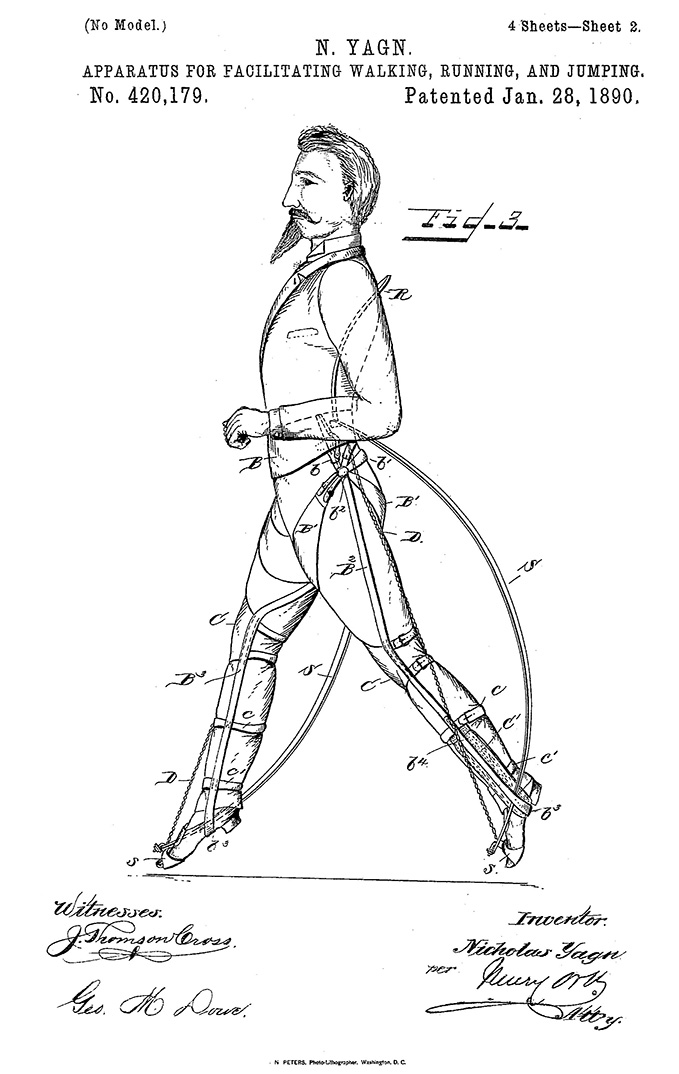
\includegraphics[width=0.8\linewidth]{chap11/11_17}
	\caption{十九世纪尼古拉斯$\cdot$杨(Nicholas Y agn)发明专利插图\cite{yagnapparatus}。 \label{fig:11_17}}
\end{figure}


第一台动力外骨骼直到20世纪60年代才被制造出来,而这项技术又经过了40年的发展才达到实际应用的程度。
如今,支架和动力外骨骼可以改善中风或脊髓损伤后的活动能力(图~\ref{fig:11_18}),支撑和稳定身体以防止受伤,并赋予使用者超人的力量。
从构思到成功实施,这段约70年的时间反映了设计、制造和测试与复杂、精细调节的生物系统和谐互动的设备的巨大挑战。


\begin{figure}[!htb]
	\centering
	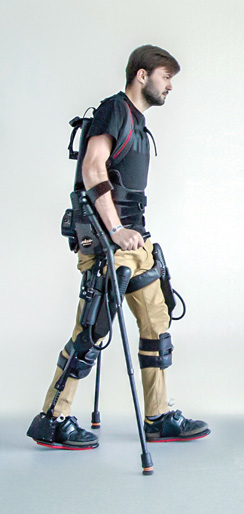
\includegraphics[width=0.4\linewidth]{chap11/11_18}
	\caption{首批帮助中风和脊髓损伤患者恢复双足运动能力的外骨骼之一。图片由 Ekso Bionics 提供。 \label{fig:11_18}}
\end{figure}


设备设计师们的共同目标是降低无损伤行走的代谢成本——考虑到自然步态的效率,这无疑是一项颇具挑战性的任务。
设计师们利用物理原型和相对简单的数学模型取得了一些进展。
菲利普$\cdot$马尔科姆(Philippe Malcolm)及其同事于2013年报告了首个能够降低行走代谢成本的外骨骼。
他们的设备佩戴在小腿上,利用连接到鞋子(并连接到空气压缩机)的气动肌肉在站立后期施加踝关节跖屈力矩。
马尔科姆报告称,与自然行走相比,该设备节省了约6\%的代谢成本。


次年,卢克$\cdot$穆尼(Luke Mooney)及其同事报告称,他们使用一种采用类似辅助策略的动力驱动但不受束缚的设备,实现了约10\%的节能效果。
2015年,史蒂夫$\cdot$柯林斯(Steve Collins)及其同事利用一种无动力踝关节外骨骼实现了同样的效果,这引发了一项颇具启发性的设想:
理论上,人体结构可以进一步进化,从而在行走过程中更加高效。
他们的设备采用被动离合机构,使与小腿肌肉平行作用的弹簧啮合和分离,从而将代谢成本降低了约7\%。
这种辅助策略利用了这样一个事实:与肌肉不同,被紧握的绳索在张力作用下无需能量即可维持其长度。


尽管取得了这些令人惊叹的成就,但设备设计的实验方法仍受到诸多限制。
例如,构建物理原型可能成本高昂且耗时,而且仅凭实验——即在不了解肌肉力量或肌肉能量消耗的情况下——很难深入了解肌肉骨骼系统与辅助设备之间的相互作用。


肌肉驱动模拟可用于探索新的辅助策略,而无需构建物理原型。
模拟还可用于测试假设的理想设备——这些设备没有质量,可以无损地将扭矩传输到肢体,并且没有扭矩或功率限制。
因此,我们可以使用理想设备的模拟来比较独立于其他实际挑战的辅助策略。
例如,Chris Dembia 及其同事生成了肌肉驱动的负重行走模拟,并预测了七种理想辅助设备在负重任务中的有效性(图~\ref{fig:11_19})。
虽然迄今为止,施加踝关节跖屈扭矩的装置已受到广泛关注,但其他辅助策略(例如,辅助髋关节屈曲和外展)可以提供更大的代谢节省,同时还需要更少的执行器功率。


\begin{figure}[!htb]
	\centering
	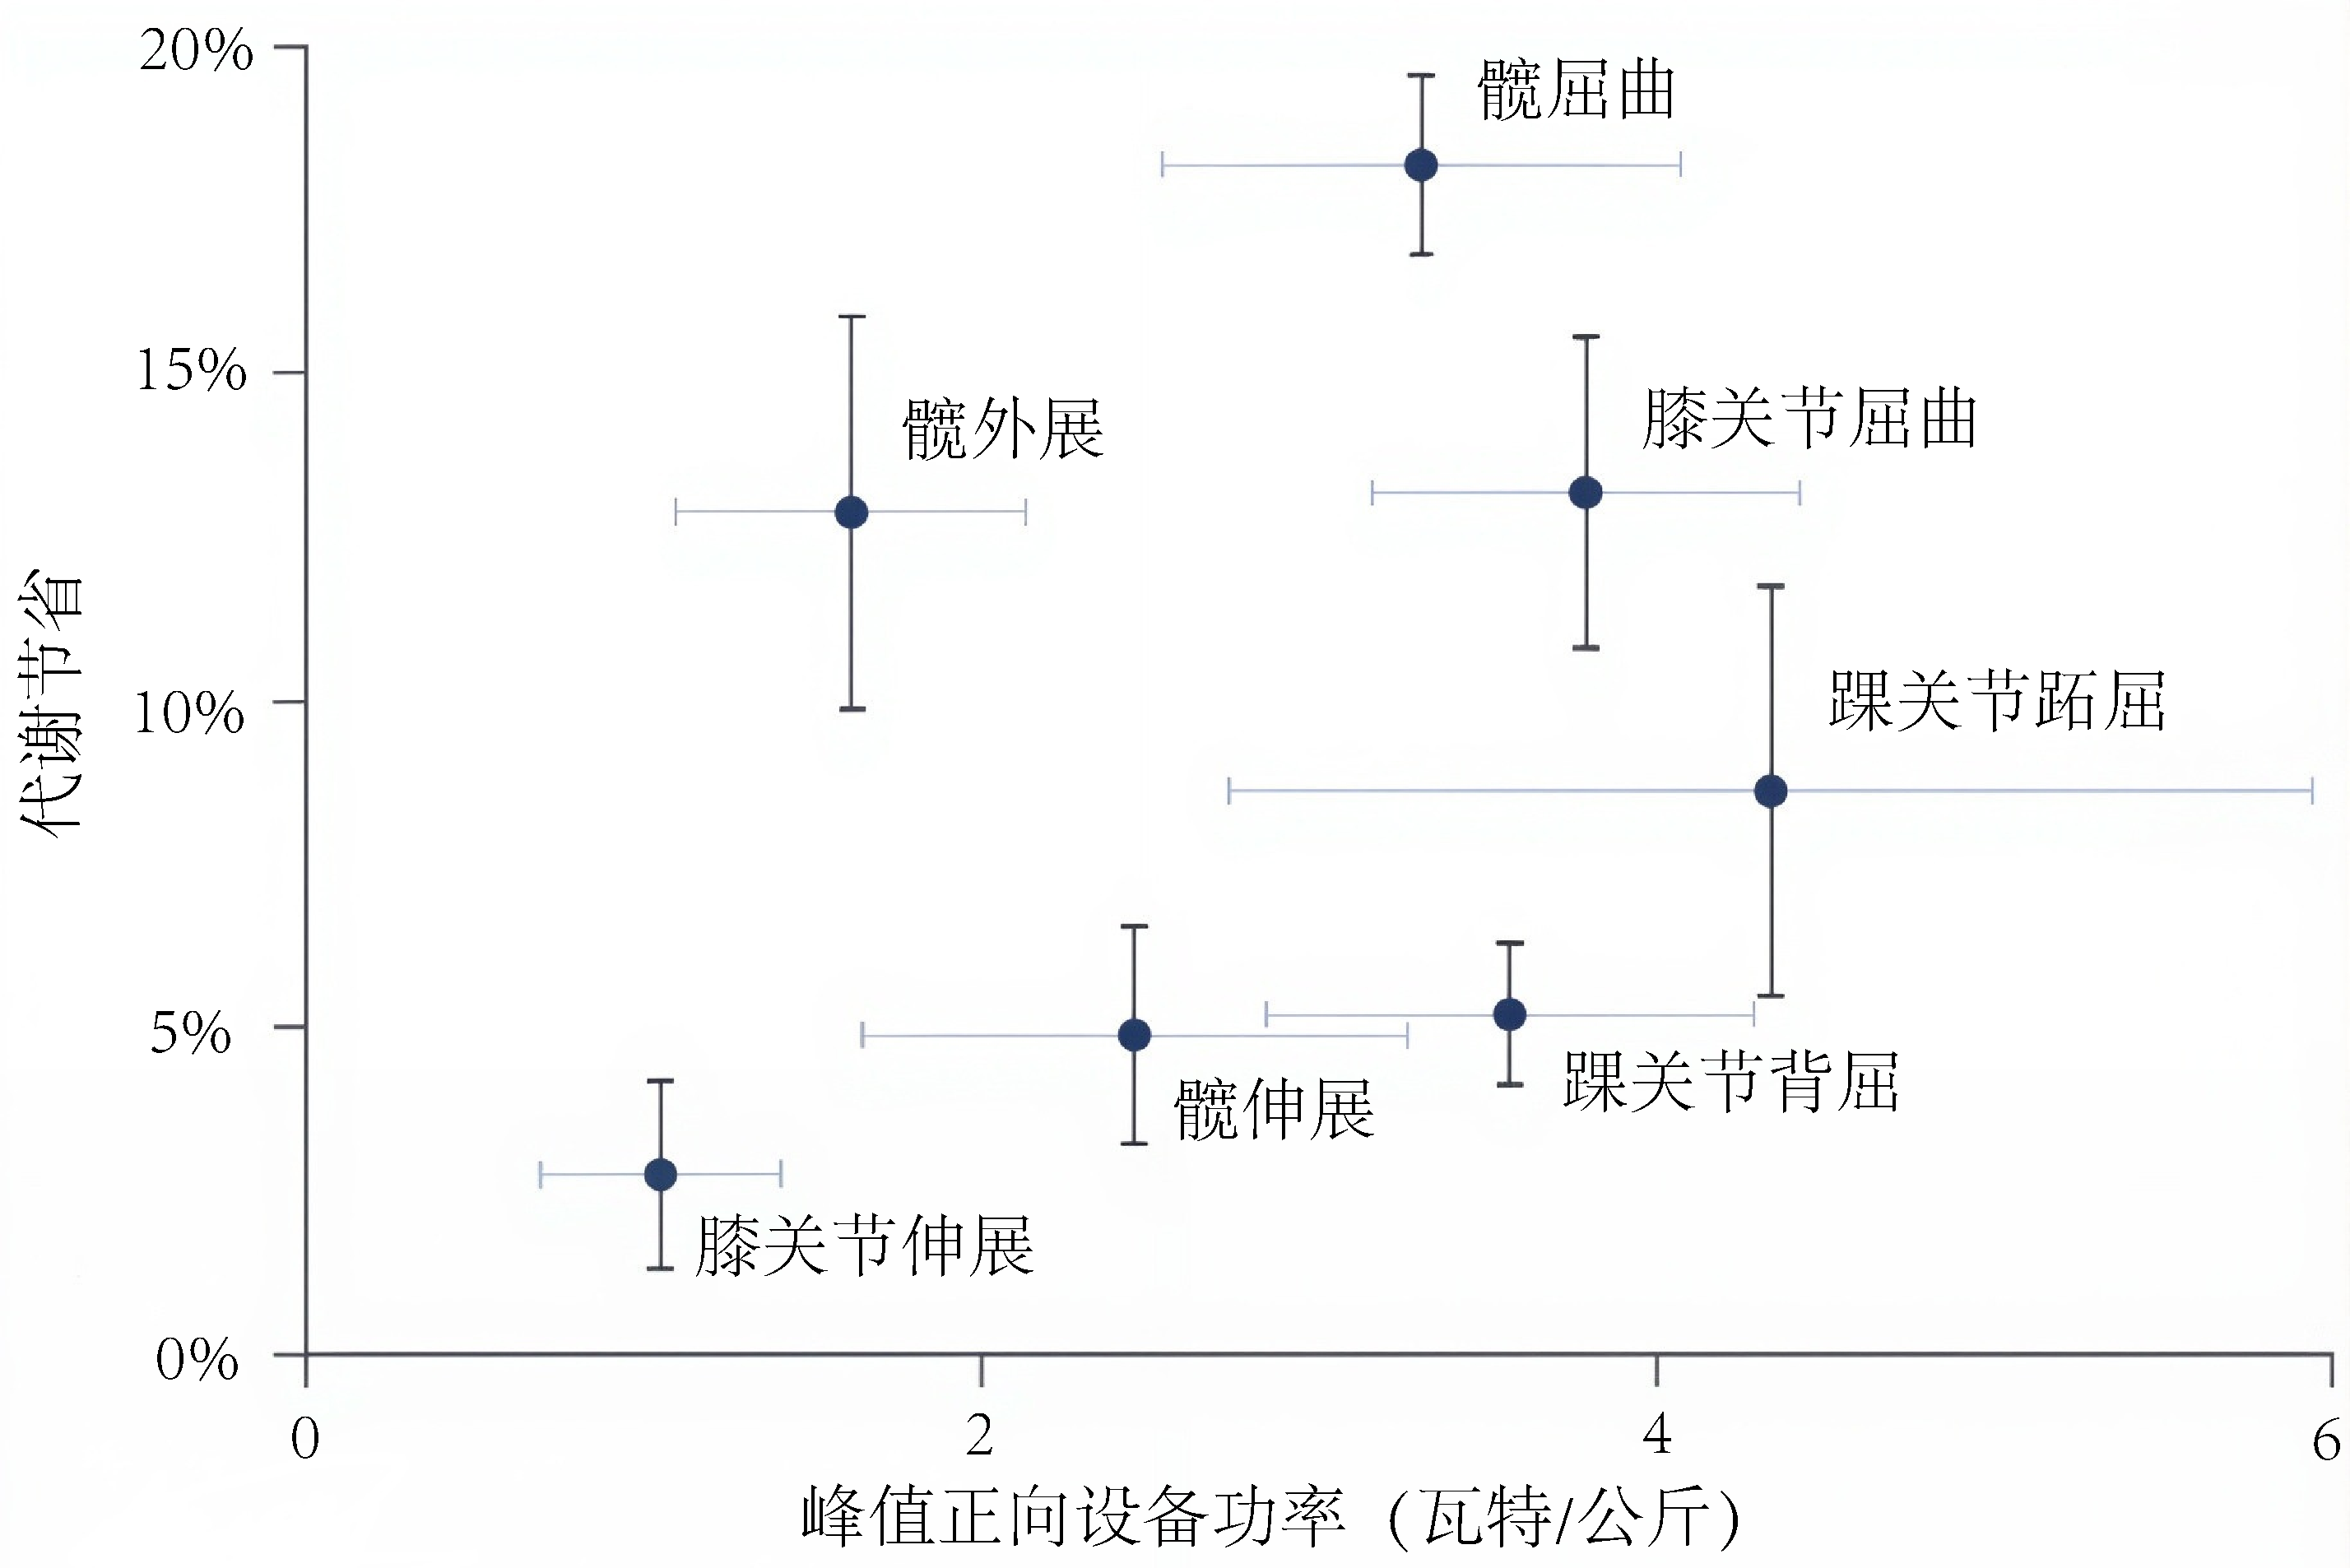
\includegraphics[width=0.8\linewidth]{chap11/11_19}
	\caption{肌肉驱动模拟预测了七种理想设备在负重 38 公斤时辅助行走的性能。
		最有前景的设备是那些节能效果显著且功耗较低的设备\cite{dembia2017simulating}。 \label{fig:11_19}}
\end{figure}


肌肉驱动模拟通过提供肌肉水平动力学和能量消耗的详细分析,补充了实验。
Chris 发现,通常情况下,最佳装置扭矩曲线与无辅助步态下肌肉产生的净关节力矩不同。
例如,理想的踝关节跖屈装置施加的扭矩在步态周期后期达到峰值,其大小仅为无辅助时肌肉产生的踝关节力矩的一半左右(图~\ref{fig:11_20})。
踝关节跖屈装置完成了比目鱼肌的大部分工作,但腓肠肌由于其对所需膝关节屈曲力矩的贡献而保持活跃。辅助装置会影响整个肢体的肌肉活动;
肌肉驱动模拟可以为这些影响提供生物力学解释,并有助于确定最佳辅助扭矩的时机和大小。
计算机辅助设计已经彻底改变了从家用电器到飞机等各种产品的工程流程;
它在加速外骨骼开发方面也具有类似的潜力。


\begin{figure}[!htb]
	\centering
	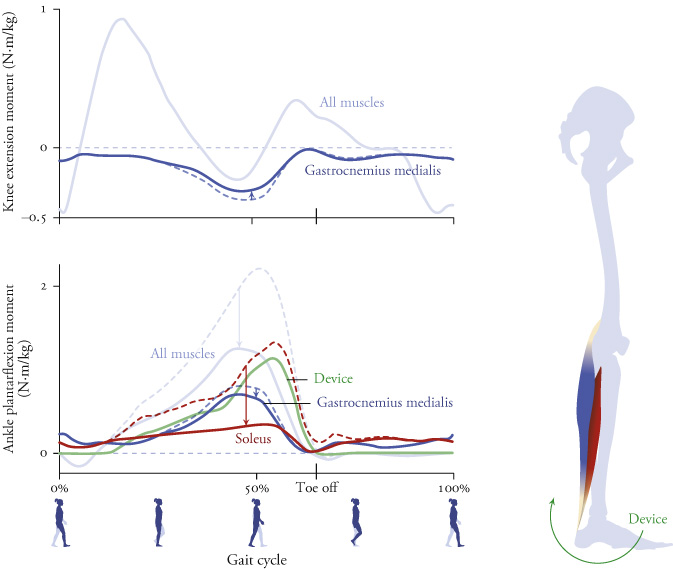
\includegraphics[width=1.0\linewidth]{chap11/11_20}
	\caption{用于辅助负重行走的踝关节跖屈装置的肌肉水平分析(7位受试者的平均值)。
		我们的模拟预测了无辅助(虚线)和辅助(实线)时关节力矩的差异,比目鱼肌的减少幅度远大于腓肠肌\cite{dembia2017simulating}。 \label{fig:11_20}}
\end{figure}






